\documentclass[12pt, a4paper]{article}

% ─── Packages ───────────────────────────────────────────────────────────────
\usepackage[utf8]{inputenc}
\usepackage[T1]{fontenc}
\usepackage{lmodern}
\usepackage[margin=1in]{geometry}
\usepackage{graphicx}
\usepackage{xcolor}
\usepackage{hyperref}
\usepackage{listings}
\usepackage{booktabs}
\usepackage{longtable}
\usepackage{enumitem}
\usepackage{amsmath}
\usepackage{fancyhdr}
\usepackage{titlesec}
\usepackage{tocloft}
\usepackage{parskip}
\usepackage{float}
\usepackage{tabularx}
\usepackage{array}
\usepackage{multirow}
\usepackage{textcomp}
\usepackage{tikz}
\usetikzlibrary{arrows.meta, positioning, shapes.geometric, fit, calc, backgrounds, decorations.pathreplacing}
\usepackage{pgfplots}
\pgfplotsset{compat=1.18}

% ─── Colors ─────────────────────────────────────────────────────────────────
\definecolor{primary}{HTML}{0984E3}
\definecolor{dark}{HTML}{2D3436}
\definecolor{codebg}{HTML}{F5F6FA}
\definecolor{codeframe}{HTML}{DFE6E9}
\definecolor{linkblue}{HTML}{0984E3}
\definecolor{sectionblue}{HTML}{0652DD}
\definecolor{keywordgreen}{HTML}{00B894}
\definecolor{stringorange}{HTML}{E17055}
\definecolor{commentgray}{HTML}{636E72}

% ─── Hyperref Setup ─────────────────────────────────────────────────────────
\hypersetup{
    colorlinks=true,
    linkcolor=sectionblue,
    urlcolor=linkblue,
    citecolor=primary,
    pdftitle={PolicyCapture Local -- Deployment \& Implementation Guide},
    pdfauthor={PolicyCapture Team},
    pdfsubject={Technical Documentation},
}

% ─── Code Listing Style ────────────────────────────────────────────────────
\lstdefinestyle{basestyle}{
    backgroundcolor=\color{codebg},
    basicstyle=\ttfamily\small,
    breaklines=true,
    breakatwhitespace=false,
    frame=single,
    rulecolor=\color{codeframe},
    framesep=6pt,
    xleftmargin=8pt,
    xrightmargin=8pt,
    showstringspaces=false,
    tabsize=2,
    captionpos=b,
    aboveskip=12pt,
    belowskip=8pt,
}

\lstdefinestyle{bash}{
    style=basestyle,
    language=bash,
    keywordstyle=\color{primary}\bfseries,
    stringstyle=\color{stringorange},
    commentstyle=\color{commentgray}\itshape,
    morekeywords={brew,apt,pip,python,curl,uvicorn,gunicorn,tesseract,git,source,mkdir,cd,lsof,kill,ffmpeg},
}

\lstdefinestyle{sql}{
    style=basestyle,
    language=SQL,
    keywordstyle=\color{primary}\bfseries,
    stringstyle=\color{stringorange},
    commentstyle=\color{commentgray}\itshape,
}

\lstdefinestyle{json}{
    style=basestyle,
    keywordstyle=\color{primary},
    stringstyle=\color{stringorange},
    morestring=[b]",
}

\lstdefinestyle{python}{
    style=basestyle,
    language=Python,
    keywordstyle=\color{primary}\bfseries,
    stringstyle=\color{stringorange},
    commentstyle=\color{commentgray}\itshape,
}

\lstdefinestyle{plain}{
    style=basestyle,
}

% ─── Section Formatting ────────────────────────────────────────────────────
\titleformat{\section}
    {\Large\bfseries\color{dark}}
    {\thesection}{1em}{}[\vspace{-4pt}\textcolor{primary}{\rule{\textwidth}{1.5pt}}]

\titleformat{\subsection}
    {\large\bfseries\color{dark}}
    {\thesubsection}{1em}{}

\titleformat{\subsubsection}
    {\normalsize\bfseries\color{dark}}
    {\thesubsubsection}{1em}{}

% ─── Header/Footer ─────────────────────────────────────────────────────────
\pagestyle{fancy}
\fancyhf{}
\fancyhead[L]{\small\textcolor{commentgray}{PolicyCapture Local}}
\fancyhead[R]{\small\textcolor{commentgray}{Deployment \& Implementation Guide}}
\fancyfoot[C]{\small\textcolor{commentgray}{\thepage}}
\renewcommand{\headrulewidth}{0.4pt}
\renewcommand{\footrulewidth}{0pt}

% ─── Custom Commands ───────────────────────────────────────────────────────
\newcommand{\apimethod}[2]{\texttt{\textcolor{primary}{\textbf{#1}} #2}}
\newcommand{\codeinline}[1]{\texttt{\small\colorbox{codebg}{#1}}}
\newcommand{\filepath}[1]{\texttt{\small #1}}

% ─── Additional Colors for Diagrams ────────────────────────────────────────
\definecolor{browserfill}{HTML}{DFE6E9}
\definecolor{serverfill}{HTML}{74B9FF}
\definecolor{pipelinefill}{HTML}{55EFC4}
\definecolor{storagefill}{HTML}{FFEAA7}
\definecolor{uifill}{HTML}{A29BFE}
\definecolor{arrowgray}{HTML}{636E72}
\definecolor{rejectred}{HTML}{D63031}
\definecolor{acceptgreen}{HTML}{00B894}
\definecolor{warnamber}{HTML}{FDCB6E}
\definecolor{threadfill}{HTML}{FAB1A0}
\definecolor{dbfill}{HTML}{81ECEC}

% ─── TikZ Styles ───────────────────────────────────────────────────────────
\tikzset{
    sysblock/.style={
        rectangle, rounded corners=4pt, draw=#1!60!black, fill=#1!25,
        minimum width=2.8cm, minimum height=1cm,
        font=\small\sffamily, text=dark, align=center,
        line width=0.6pt
    },
    sysblock/.default=primary,
    tierbox/.style={
        rectangle, rounded corners=6pt, draw=#1!50!black, fill=#1!8,
        line width=1pt, inner sep=10pt
    },
    tierbox/.default=primary,
    tierlab/.style={
        font=\small\sffamily\bfseries, text=dark
    },
    pipenode/.style={
        rectangle, rounded corners=3pt, draw=primary!70, fill=pipelinefill!30,
        minimum width=2cm, minimum height=0.7cm,
        font=\scriptsize\sffamily, align=center, line width=0.5pt
    },
    dataarrow/.style={
        -{Stealth[length=5pt]}, line width=0.8pt, color=arrowgray
    },
    bigarrow/.style={
        -{Stealth[length=7pt]}, line width=1.2pt, color=primary
    },
    dasharrow/.style={
        -{Stealth[length=5pt]}, line width=0.6pt, dashed, color=commentgray
    },
    storagenode/.style={
        cylinder, draw=storagefill!60!black, fill=storagefill!40,
        shape border rotate=90, aspect=0.3,
        minimum width=1.8cm, minimum height=1cm,
        font=\scriptsize\sffamily, align=center, line width=0.5pt
    },
    decisionnode/.style={
        diamond, draw=primary!70, fill=primary!10,
        minimum width=1.5cm, minimum height=1cm,
        font=\scriptsize\sffamily, align=center, inner sep=1pt
    },
}

% ─── Document ──────────────────────────────────────────────────────────────
\begin{document}

% ─── Title Page ────────────────────────────────────────────────────────────
\begin{titlepage}
    \centering
    \vspace*{2cm}

    {\Huge\bfseries\textcolor{dark}{PolicyCapture Local}\par}
    \vspace{0.5cm}
    {\LARGE\textcolor{primary}{Deployment \& Implementation Guide}\par}

    \vspace{1.5cm}
    \textcolor{primary}{\rule{0.6\textwidth}{2pt}}
    \vspace{1.5cm}

    {\large
    \begin{tabular}{rl}
        \textbf{Version:} & 0.1.0 \\
        \textbf{Last Updated:} & March 2026 \\
        \textbf{Platform:} & macOS / Linux \\
        \textbf{Runtime:} & Python 3.11+ / FastAPI / Uvicorn \\
        \textbf{Database:} & SQLite (WAL mode) \\
        \textbf{Server:} & \texttt{localhost:8420} \\
    \end{tabular}
    }

    \vspace{2cm}

    {\large\textcolor{commentgray}{Local-first extraction workflow for recorded screen sessions.\\
    Process policy/benefits system reviews into structured evidence documentation.}\par}

    \vfill
    {\small\textcolor{commentgray}{Confidential --- Contains system architecture and implementation details}\par}
\end{titlepage}

% ─── Table of Contents ─────────────────────────────────────────────────────
\newpage
\tableofcontents
\newpage

% ════════════════════════════════════════════════════════════════════════════
\section{What Is PolicyCapture Local?}
% ════════════════════════════════════════════════════════════════════════════

PolicyCapture Local is a \textbf{local-first} screen recording and document extraction platform. It is purpose-built for \textbf{policy and benefits system review workflows} --- the kind where a reviewer walks through a government benefits portal (Medicaid, SNAP, TANF, etc.), captures their screen session, and needs to produce structured, evidence-style documentation from what they saw.

\subsection{The Problem It Solves}

Manually screenshotting dozens of pages, organizing them, and writing up findings is tedious and error-prone. PolicyCapture automates the mechanical parts:

\begin{itemize}
    \item Records the screen session as video
    \item Extracts the most informative frames automatically
    \item Runs OCR and entity recognition on those frames
    \item Generates a structured HTML evidence report
\end{itemize}

\subsection{The Key Design Constraint}

Everything runs locally. No cloud APIs, no external services, no data leaves the machine. This is non-negotiable because the content being captured (benefits applications, SSNs, income data) is sensitive PII.

% ════════════════════════════════════════════════════════════════════════════
\section{Why This Architecture?}
% ════════════════════════════════════════════════════════════════════════════

\subsection{Local-First}

All processing happens on \codeinline{localhost:8420}. The SQLite database, video files, extracted frames, and reports all live in the \codeinline{data/} directory on the user's machine. There is no authentication layer because there is no network exposure --- the server binds to \codeinline{0.0.0.0:8420} for local access only.

\subsection{Modular Pipeline}

Each processing stage (frame extraction, blur detection, OCR, entity recognition, etc.) is a standalone Python module in \filepath{packages/core/pipeline/}. This means:

\begin{itemize}
    \item Stages can be tested independently
    \item Stages can be replaced (e.g., swap regex NER for a trained model) without touching anything else
    \item The pipeline can be run partially (e.g., extract frames without running OCR)
\end{itemize}

\subsection{No ML Dependencies in Core}

The core pipeline deliberately avoids heavy ML frameworks. OCR uses Tesseract (a system binary), entity extraction uses regex, and classification uses keyword rules. This keeps the install footprint small and startup instant. ML-based alternatives are marked as extension points in the code.

\subsection{Why FastAPI + Vanilla JS (Not React/Next.js)?}

\begin{itemize}
    \item \textbf{FastAPI} gives us async endpoints, automatic OpenAPI docs, Pydantic validation, and Jinja2 template rendering --- all in one lightweight package
    \item \textbf{Vanilla JS} avoids a build step, \codeinline{node\_modules}, and framework churn. The UI is a review tool, not a SaaS product --- it doesn't need React's component model
    \item \textbf{Jinja2 templates} give us server-rendered pages where it matters (recorder, frame review, OCR review) while \codeinline{app.js} provides a lightweight SPA for the dashboard
\end{itemize}

% ════════════════════════════════════════════════════════════════════════════
\section{System Design Decisions --- Alternatives Considered}
% ════════════════════════════════════════════════════════════════════════════

Every architectural choice in PolicyCapture was made against a specific set of constraints: \textbf{PII sensitivity}, \textbf{zero-internet deployment}, \textbf{single-user local use}, and \textbf{minimal install friction}. This section documents what we chose, what we considered, and why we decided the way we did.

\subsection{Web Framework: FastAPI vs.\ Flask vs.\ Django}

\begin{figure}[H]
\centering
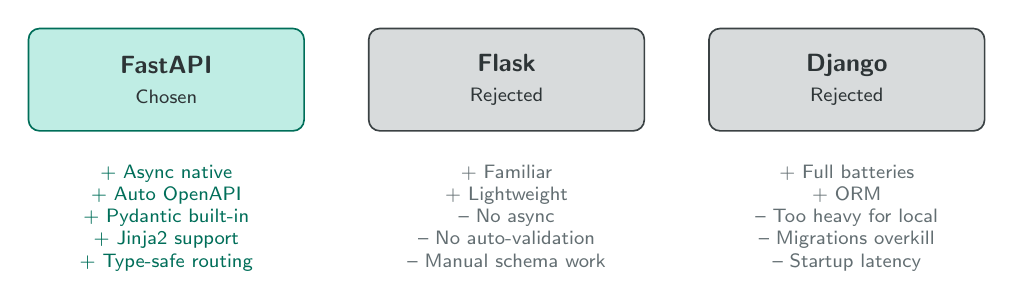
\begin{tikzpicture}
    \node[sysblock=acceptgreen, minimum width=3.5cm, minimum height=1.3cm] (fastapi) {\textbf{FastAPI}\\\scriptsize Chosen};
    \node[sysblock=commentgray, minimum width=3.5cm, minimum height=1.3cm, right=0.8cm of fastapi] (flask) {\textbf{Flask}\\\scriptsize Rejected};
    \node[sysblock=commentgray, minimum width=3.5cm, minimum height=1.3cm, right=0.8cm of flask] (django) {\textbf{Django}\\\scriptsize Rejected};

    \node[font=\scriptsize\sffamily, text=acceptgreen!60!black, below=0.3cm of fastapi, align=center] {+ Async native\\+ Auto OpenAPI\\+ Pydantic built-in\\+ Jinja2 support\\+ Type-safe routing};
    \node[font=\scriptsize\sffamily, text=commentgray, below=0.3cm of flask, align=center] {+ Familiar\\+ Lightweight\\-- No async\\-- No auto-validation\\-- Manual schema work};
    \node[font=\scriptsize\sffamily, text=commentgray, below=0.3cm of django, align=center] {+ Full batteries\\+ ORM\\-- Too heavy for local\\-- Migrations overkill\\-- Startup latency};
\end{tikzpicture}
\end{figure}

\textbf{Decision rationale:} FastAPI gives us async request handling (critical when serving video/image files while processing runs in background threads), automatic request validation via Pydantic models, and built-in OpenAPI documentation --- all without the weight of Django's ORM, admin panel, and migration system that we don't need for a single-file SQLite database.

\subsection{Database: SQLite vs.\ PostgreSQL vs.\ File-Based JSON}

\begin{longtable}{@{} p{3cm} p{3.5cm} p{3.5cm} p{3.5cm} @{}}
    \toprule
    \textbf{Criterion} & \textbf{SQLite (chosen)} & \textbf{PostgreSQL} & \textbf{JSON files} \\
    \midrule
    Install complexity & Zero (built into Python) & Requires server process & Zero \\
    Relational queries & Full SQL & Full SQL & Manual \\
    Concurrent access & WAL mode handles it & Native & Race conditions \\
    Backup & Copy one file & pg\_dump & Copy directory \\
    Schema evolution & ALTER TABLE & Migrations (Alembic) & No schema \\
    Data integrity & Foreign keys, constraints & Full ACID & None \\
    \midrule
    \textbf{Verdict} & \textcolor{acceptgreen}{\textbf{Chosen}} & Overkill for local & Too fragile \\
    \bottomrule
\end{longtable}

\textbf{Why not PostgreSQL?} The application is single-user, runs on localhost, and needs zero-configuration deployment. Installing and configuring a Postgres server would violate the ``download and run'' constraint. SQLite with WAL mode gives us concurrent reads (the API serving frames while the pipeline writes new ones) without any server process.

\textbf{Why not flat JSON files?} With 5 related entity types (jobs, frames, screenshots, sections, reports) and queries like ``get all frames for job X where relevance $> 0.3$'', a relational model is essential. JSON files would require loading entire datasets into memory and implementing ad-hoc filtering.

\subsection{OCR: Tesseract (subprocess) vs.\ PaddleOCR vs.\ Cloud APIs}

\begin{longtable}{@{} p{3.5cm} p{3.5cm} p{3.5cm} p{3.5cm} @{}}
    \toprule
    \textbf{Criterion} & \textbf{Tesseract (chosen)} & \textbf{PaddleOCR} & \textbf{Azure/AWS OCR} \\
    \midrule
    Accuracy & Good (with preprocessing) & Better on complex layouts & Best \\
    Install size & $\sim$30\,MB binary & $\sim$1.5\,GB (ML models) & Zero (cloud) \\
    Latency & 50--200\,ms/frame & 200--500\,ms/frame & 500--2000\,ms (network) \\
    Internet required & No & No & \textcolor{rejectred}{\textbf{Yes}} \\
    PII exposure risk & None (local) & None (local) & \textcolor{rejectred}{\textbf{Data leaves machine}} \\
    Python deps & None (subprocess) & torch, paddlepaddle & SDK only \\
    \midrule
    \textbf{Verdict} & \textcolor{acceptgreen}{\textbf{Chosen}} & Optional upgrade & Disqualified (PII) \\
    \bottomrule
\end{longtable}

\textbf{Key insight:} Tesseract is called as a \textbf{subprocess}, not via \codeinline{pytesseract}. This eliminates the pandas/PIL transitive dependency chain and lets us parse TSV output directly. The multi-strategy preprocessing (standard, Otsu, adaptive, heavy) compensates for Tesseract's weaker handling of complex layouts.

\subsection{NER: Regex vs.\ SpaCy vs.\ GLiNER vs.\ LLM}

\begin{longtable}{@{} p{3cm} p{3cm} p{3cm} p{3cm} p{2cm} @{}}
    \toprule
    & \textbf{Regex (chosen)} & \textbf{SpaCy} & \textbf{GLiNER} & \textbf{LLM API} \\
    \midrule
    Install size & 0\,MB & $\sim$400\,MB & $\sim$800\,MB & 0 (cloud) \\
    Speed & $<$10\,ms & $\sim$50\,ms & $\sim$200\,ms & $\sim$2\,s \\
    PII types & 20+ custom & Generic NER & Custom labels & Any \\
    Deterministic & Yes & Mostly & No & No \\
    Offline & Yes & Yes & Yes & No \\
    \midrule
    \textbf{Verdict} & \textcolor{acceptgreen}{\textbf{Chosen}} & Good upgrade & Good upgrade & Disqualified \\
    \bottomrule
\end{longtable}

\textbf{Why regex?} Our entity types are \textit{highly structured} (SSN = \codeinline{XXX-XX-XXXX}, EIN = \codeinline{XX-XXXXXXX}, dates in known formats). Regex gives 100\% precision on these patterns, runs in under 10\,ms, adds zero install weight, and produces deterministic results that reviewers can trust. SpaCy and GLiNER are marked as upgrade paths for entities that require contextual understanding (e.g., distinguishing a person's name from an organization).

\subsection{Frontend: Vanilla JS vs.\ React vs.\ Svelte}

\begin{longtable}{@{} p{3cm} p{4cm} p{3.5cm} p{3.5cm} @{}}
    \toprule
    & \textbf{Vanilla JS (chosen)} & \textbf{React} & \textbf{Svelte} \\
    \midrule
    Build step & None & Required (Webpack/Vite) & Required (Vite) \\
    Bundle size & 0\,KB overhead & $\sim$140\,KB (React+DOM) & $\sim$10\,KB \\
    Node.js required & No & Yes & Yes \\
    Component reuse & Manual DOM helpers & JSX components & .svelte files \\
    Learning curve & Zero (web standards) & Moderate & Low \\
    \midrule
    \textbf{Verdict} & \textcolor{acceptgreen}{\textbf{Chosen}} & Overkill & Good alternative \\
    \bottomrule
\end{longtable}

\textbf{Decision rationale:} PolicyCapture's UI has exactly 4 pages. Adding a Node.js toolchain, a bundler, and a framework runtime for 4 pages would be over-engineering. Vanilla JS with Jinja2 templates gives us server-rendered initial loads (good for SEO-irrelevant but fast-feeling local tools), zero build step, and instant deployability. The \codeinline{app.js} file implements a minimal hash router ($\sim$30 lines) that handles the dashboard SPA views.

\subsection{Video Processing: OpenCV vs.\ FFmpeg vs.\ MoviePy}

\begin{longtable}{@{} p{3.5cm} p{4cm} p{4cm} p{3cm} @{}}
    \toprule
    & \textbf{OpenCV (chosen)} & \textbf{FFmpeg (subprocess)} & \textbf{MoviePy} \\
    \midrule
    Frame extraction & \codeinline{VideoCapture} API & \codeinline{-vf fps=2} filter & clip.iter\_frames() \\
    Image analysis & Built-in (SSIM, blur, etc.) & Not available & Requires OpenCV anyway \\
    WebM support & Yes (with quirks) & Excellent & Via FFmpeg \\
    Install & pip (headless, $\sim$40\,MB) & System binary & pip (pulls FFmpeg) \\
    Timestamp seeking & \codeinline{CAP\_PROP\_POS\_MSEC} & \codeinline{-ss} flag & Via FFmpeg \\
    \midrule
    \textbf{Verdict} & \textcolor{acceptgreen}{\textbf{Chosen}} & Good for transcoding & Unnecessary layer \\
    \bottomrule
\end{longtable}

\textbf{Why OpenCV?} We need frame extraction \textit{and} image analysis (blur detection, SSIM, histogram correlation, edge detection, Hough transforms) in the same pipeline. OpenCV does both. Using FFmpeg for extraction and OpenCV for analysis would mean two video decoders and a serialization boundary between them. The \codeinline{opencv-python-headless} package avoids pulling in GUI dependencies (Qt/GTK).

\subsection{Concurrency Model: Threading vs.\ Asyncio vs.\ Celery}

\begin{figure}[H]
\centering
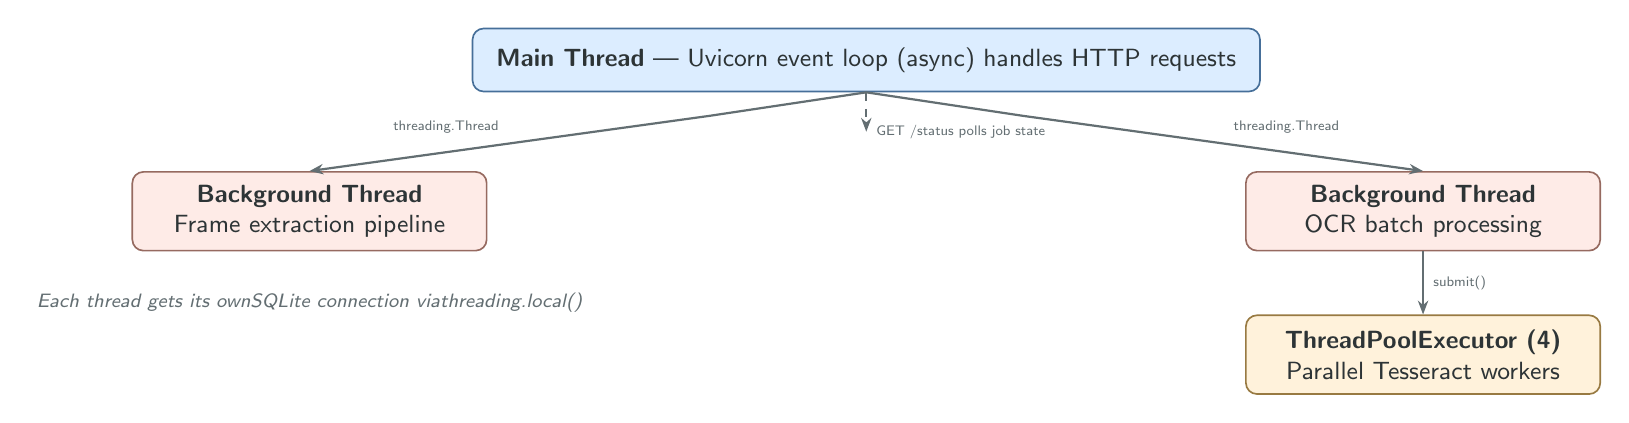
\begin{tikzpicture}[node distance=0.5cm and 0.3cm]

    % Main thread
    \node[sysblock=serverfill, minimum width=10cm, minimum height=0.8cm] (main) {\textbf{Main Thread} --- Uvicorn event loop (async) handles HTTP requests};

    % Worker threads
    \node[sysblock=threadfill, minimum width=4.5cm, below left=1cm and -0.2cm of main] (bg1) {\textbf{Background Thread}\\Frame extraction pipeline};
    \node[sysblock=threadfill, minimum width=4.5cm, below right=1cm and -0.2cm of main] (bg2) {\textbf{Background Thread}\\OCR batch processing};

    % Thread pool
    \node[sysblock=warnamber, minimum width=4.5cm, below=0.8cm of bg2] (pool) {\textbf{ThreadPoolExecutor (4)}\\Parallel Tesseract workers};

    % Arrows
    \draw[dataarrow] (main.south) -- ++(-2,-0.3) -- (bg1.north) node[midway, above left, font=\tiny\sffamily] {threading.Thread};
    \draw[dataarrow] (main.south) -- ++(2,-0.3) -- (bg2.north) node[midway, above right, font=\tiny\sffamily] {threading.Thread};
    \draw[dataarrow] (bg2.south) -- (pool.north) node[midway, right, font=\tiny\sffamily] {submit()};

    % DB access note
    \node[font=\scriptsize\sffamily\itshape, text=commentgray, below=0.4cm of bg1] {Each thread gets its own\\SQLite connection via\\threading.local()};

    % Status polling
    \draw[dasharrow] (main.south) -- ++(0,-0.5) node[right, font=\tiny\sffamily, text=commentgray] {GET /status polls job state};

\end{tikzpicture}
\caption{Concurrency model. Long operations run in background threads; the async main loop stays responsive.}
\end{figure}

\textbf{Why not Celery/Redis?} Celery requires a message broker (Redis or RabbitMQ) --- another process to install and manage. For a single-user local tool that processes one video at a time, \codeinline{threading.Thread} is sufficient. The background thread updates job status in SQLite; the frontend polls \codeinline{GET /api/jobs/\{id\}/status} at 1-second intervals.

\textbf{Why not pure asyncio?} OpenCV's \codeinline{VideoCapture} and Tesseract's subprocess calls are blocking I/O. Running them in the async event loop would block all other requests. Background threads with \codeinline{threading.Thread} let these CPU/IO-bound operations run without starving the HTTP server.

\textbf{Thread safety for SQLite:} Each thread gets its own connection via \codeinline{threading.local()}. SQLite's WAL mode allows concurrent readers + one writer. The pipeline thread writes frames/screenshots while the API thread reads them for status updates --- WAL handles this without locks.

\subsection{Report Format: Self-Contained HTML vs.\ PDF vs.\ DOCX}

\begin{itemize}
    \item \textbf{Self-contained HTML (chosen):} Images embedded as base64 data URIs. One file, opens in any browser, no external dependencies. File size is larger ($\sim$5--20\,MB) but portability is perfect.
    \item \textbf{PDF:} Better for print/archive. Stubbed in \filepath{generate\_report.py} as a future extension. ReportLab or weasyprint would convert the HTML.
    \item \textbf{DOCX:} Editable but requires python-docx, complex formatting, and doesn't render images as cleanly.
\end{itemize}

\subsection{Scene Detection: Two-Pass Hybrid vs.\ Pure SSIM vs.\ Deep Learning}

The two-pass approach (perceptual hash pre-filter + SSIM on ambiguous cases) is a deliberate optimization:

\begin{figure}[H]
\centering
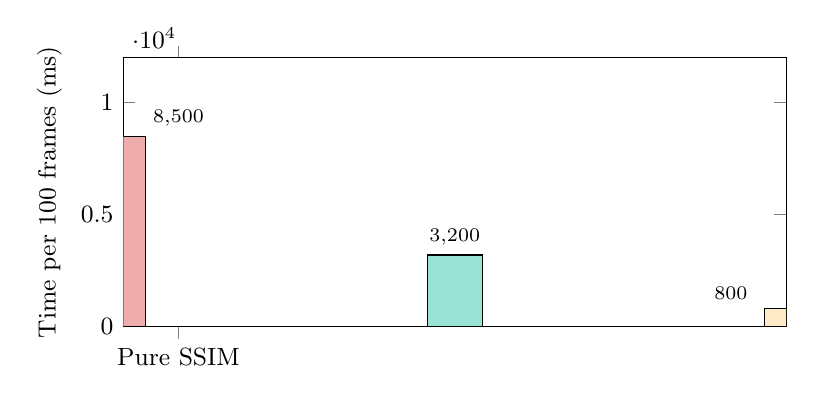
\begin{tikzpicture}
\begin{axis}[
    width=10cm, height=5cm,
    ybar,
    bar width=20pt,
    ylabel={Time per 100 frames (ms)},
    symbolic x coords={Pure SSIM, Two-Pass Hybrid, Pure pHash},
    xtick=data,
    nodes near coords,
    nodes near coords align={vertical},
    ymin=0, ymax=12000,
    ylabel style={font=\small},
    xlabel style={font=\small},
    tick label style={font=\small},
    every node near coord/.style={font=\scriptsize},
]
\addplot[fill=rejectred!40] coordinates {(Pure SSIM, 8500)};
\addplot[fill=acceptgreen!40] coordinates {(Two-Pass Hybrid, 3200)};
\addplot[fill=warnamber!40] coordinates {(Pure pHash, 800)};
\end{axis}
\end{tikzpicture}
\caption{Scene detection performance comparison. Pure pHash is fastest but misses subtle changes; the hybrid approach balances speed and accuracy.}
\end{figure}

Pure pHash misses gradual scrolling and subtle UI state changes. Pure SSIM is accurate but expensive. The two-pass hybrid filters out 60--80\% of obvious non-changes via pHash ($< 1$\,ms each), then spends the expensive SSIM computation ($\sim$75\,ms each) only on ambiguous frames. The adaptive threshold (\S\ref{sec:adaptive}) further tunes sensitivity based on recording activity patterns.

\subsection{Design Principle Summary}

\begin{longtable}{@{} p{4cm} p{10cm} @{}}
    \toprule
    \textbf{Principle} & \textbf{How It Manifests} \\
    \midrule
    \endhead
    Data sovereignty & All processing local; no network calls; PII never leaves the machine \\
    Zero-config deployment & SQLite (no DB server), Tesseract (single binary), pip install \\
    Modular pipeline & Each of 12 stages is a standalone .py file with a pure function interface \\
    Human-in-the-loop & Pipeline produces candidates; user reviews before OCR runs \\
    Progressive disclosure & Extract frames first, review, then OCR --- not all-at-once \\
    Graceful degradation & No Tesseract? Pipeline still extracts and scores frames. No keywords match? Structure score still works \\
    Extension over modification & ML upgrades are drop-in replacements at marked extension points \\
    \bottomrule
\end{longtable}

% ════════════════════════════════════════════════════════════════════════════
\section{Technology Stack \& Rationale}
% ════════════════════════════════════════════════════════════════════════════

\begin{longtable}{@{} p{3cm} p{4cm} p{7cm} @{}}
    \toprule
    \textbf{Layer} & \textbf{Technology} & \textbf{Rationale} \\
    \midrule
    \endhead
    Runtime & Python 3.11+ & Type hints, \codeinline{match} statements, walrus operator, fast startup \\
    Web Framework & FastAPI 0.104+ & Async, automatic OpenAPI, Pydantic integration, Jinja2 support \\
    ASGI Server & Uvicorn & Production-grade, supports \codeinline{--reload} for development \\
    Computer Vision & OpenCV (headless) 4.8+ & Industry standard for frame extraction, image processing, SSIM \\
    OCR Engine & Tesseract (subprocess) & Open-source, offline, no Python ML stack needed \\
    NER & Regex (custom) & Deterministic, fast, no model files to ship, handles PII patterns \\
    Database & SQLite (WAL mode) & Zero-config, file-based, concurrent reads, perfect for local apps \\
    Data Validation & Pydantic 2.5+ & Fast, type-safe request/response schemas \\
    Templating & Jinja2 3.1+ & Server-side rendering for multi-page UI \\
    Frontend & Vanilla JavaScript & No build step, no dependencies, instant page loads \\
    Image Processing & Pillow 10+ & Thumbnail generation, image format conversion \\
    PDF (planned) & ReportLab 4+ & Programmatic PDF generation (stub exists, not yet wired) \\
    Math & NumPy 1.25+ & Array operations for image comparison, MSE, histograms \\
    \bottomrule
\end{longtable}

\subsection{System Dependencies (Not in pip)}

\begin{tabularx}{\textwidth}{@{} l l X @{}}
    \toprule
    \textbf{Dependency} & \textbf{Required For} & \textbf{Install} \\
    \midrule
    Tesseract & OCR text extraction & \codeinline{brew install tesseract} (macOS) / \codeinline{apt install tesseract-ocr} (Ubuntu) \\
    Python 3.11+ & Runtime & \codeinline{brew install python@3.11} or pyenv \\
    \bottomrule
\end{tabularx}

% ════════════════════════════════════════════════════════════════════════════
\section{System Architecture Overview}
% ════════════════════════════════════════════════════════════════════════════

The system follows a three-tier architecture: \textbf{Browser Frontend} $\rightarrow$ \textbf{FastAPI Server} $\rightarrow$ \textbf{Filesystem + SQLite}. This section presents the architecture through multiple diagram perspectives.

\subsection{High-Level System Diagram}

\begin{figure}[H]
\centering
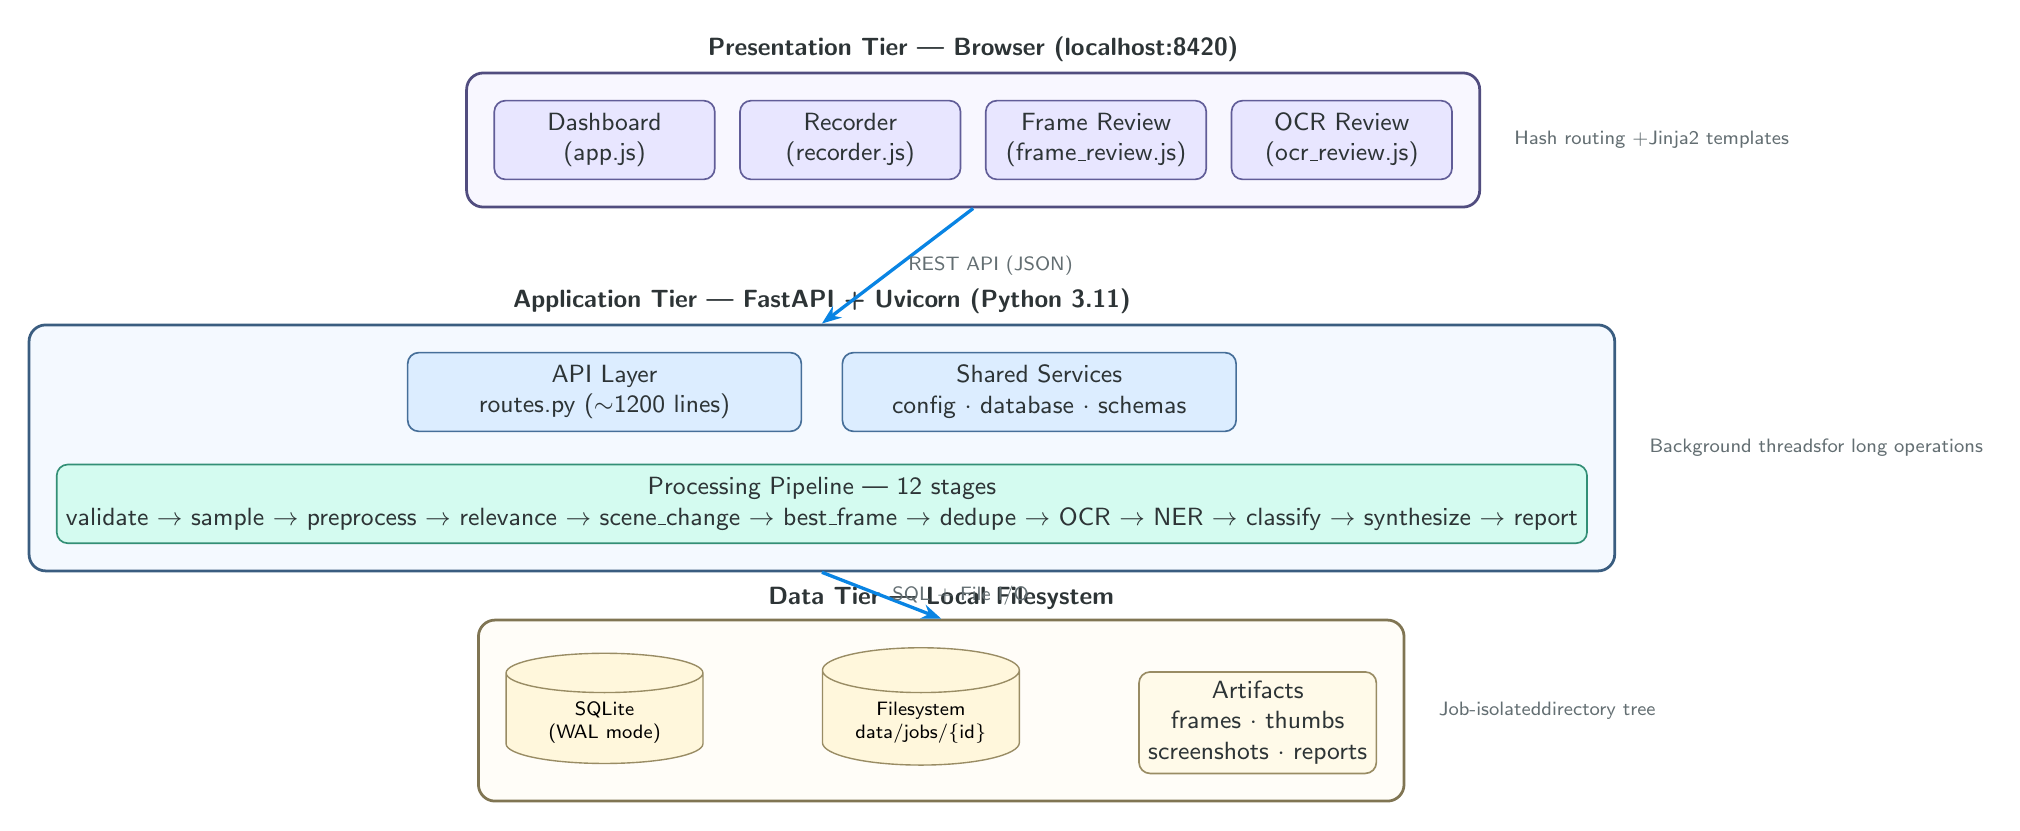
\begin{tikzpicture}[node distance=0.6cm and 0.4cm]

    % ── Browser Tier ──
    \begin{scope}[local bounding box=browsertier]
        \node[sysblock=uifill] (dash) {Dashboard\\(app.js)};
        \node[sysblock=uifill, right=0.3cm of dash] (rec) {Recorder\\(recorder.js)};
        \node[sysblock=uifill, right=0.3cm of rec] (frev) {Frame Review\\(frame\_review.js)};
        \node[sysblock=uifill, right=0.3cm of frev] (orev) {OCR Review\\(ocr\_review.js)};
    \end{scope}
    \begin{pgfonlayer}{background}
        \node[tierbox=uifill, fit=(browsertier), label={[tierlab]above:{\textcolor{dark}{Presentation Tier} --- Browser (localhost:8420)}}] (bbox) {};
    \end{pgfonlayer}

    % ── Server Tier ──
    \begin{scope}[local bounding box=servertier, shift={(0,-3.2)}]
        \node[sysblock=serverfill, minimum width=5cm] (routes) {API Layer\\routes.py ($\sim$1200 lines)};
        \node[sysblock=serverfill, minimum width=5cm, right=0.5cm of routes] (shared) {Shared Services\\config $\cdot$ database $\cdot$ schemas};
        \node[sysblock=pipelinefill, minimum width=10.5cm, below=0.4cm of $(routes.south)!0.5!(shared.south)$] (pipeline) {Processing Pipeline --- 12 stages\\validate $\rightarrow$ sample $\rightarrow$ preprocess $\rightarrow$ relevance $\rightarrow$ scene\_change $\rightarrow$ best\_frame $\rightarrow$ dedupe $\rightarrow$ OCR $\rightarrow$ NER $\rightarrow$ classify $\rightarrow$ synthesize $\rightarrow$ report};
    \end{scope}
    \begin{pgfonlayer}{background}
        \node[tierbox=serverfill, fit=(servertier), label={[tierlab]above:{\textcolor{dark}{Application Tier} --- FastAPI + Uvicorn (Python 3.11)}}] (sbox) {};
    \end{pgfonlayer}

    % ── Data Tier ──
    \begin{scope}[local bounding box=datatier, shift={(0,-7.4)}]
        \node[storagenode, minimum width=2.5cm] (db) {SQLite\\(WAL mode)};
        \node[storagenode, minimum width=2.5cm, right=1.5cm of db] (fs) {Filesystem\\data/jobs/\{id\}};
        \node[sysblock=storagefill, right=1.5cm of fs, minimum width=2.5cm] (artifacts) {Artifacts\\frames $\cdot$ thumbs\\screenshots $\cdot$ reports};
    \end{scope}
    \begin{pgfonlayer}{background}
        \node[tierbox=storagefill, fit=(datatier), label={[tierlab]above:{\textcolor{dark}{Data Tier} --- Local Filesystem}}] (dbox) {};
    \end{pgfonlayer}

    % ── Arrows ──
    \draw[bigarrow] (bbox.south) -- node[right, font=\scriptsize\sffamily, text=commentgray] {REST API (JSON)} (sbox.north);
    \draw[bigarrow] (sbox.south) -- node[right, font=\scriptsize\sffamily, text=commentgray] {SQL + File I/O} (dbox.north);

    % ── Side annotations ──
    \node[font=\scriptsize\sffamily, text=commentgray, anchor=west] at ($(bbox.east)+(0.3,0)$) {Hash routing +\\Jinja2 templates};
    \node[font=\scriptsize\sffamily, text=commentgray, anchor=west] at ($(sbox.east)+(0.3,0)$) {Background threads\\for long operations};
    \node[font=\scriptsize\sffamily, text=commentgray, anchor=west] at ($(dbox.east)+(0.3,0)$) {Job-isolated\\directory tree};

\end{tikzpicture}
\caption{Three-tier system architecture. All tiers run on localhost; no network boundary is crossed.}
\end{figure}

\subsection{Processing Pipeline Flow Diagram}

\begin{figure}[H]
\centering
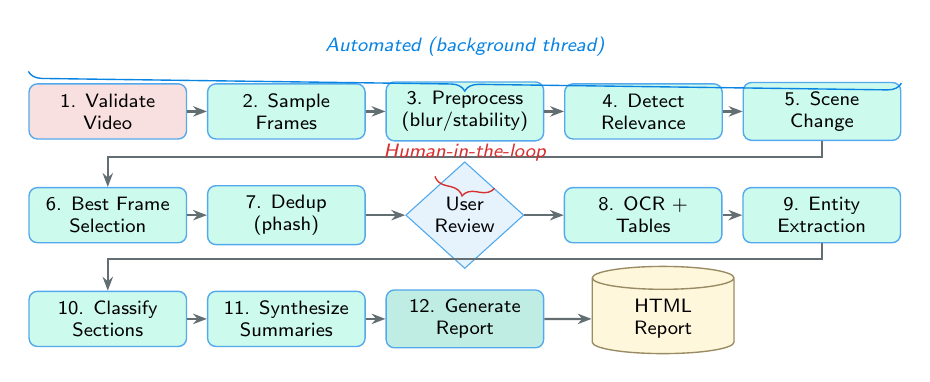
\begin{tikzpicture}[node distance=0.35cm and 0.2cm]

    % Row 1: Video input pipeline
    \node[pipenode, fill=rejectred!15] (validate) {1. Validate\\Video};
    \node[pipenode, right=0.25cm of validate] (sample) {2. Sample\\Frames};
    \node[pipenode, right=0.25cm of sample] (preprocess) {3. Preprocess\\(blur/stability)};
    \node[pipenode, right=0.25cm of preprocess] (relevance) {4. Detect\\Relevance};
    \node[pipenode, right=0.25cm of relevance] (scene) {5. Scene\\Change};

    % Row 2: Selection + OCR
    \node[pipenode, below=0.6cm of validate] (bestframe) {6. Best Frame\\Selection};
    \node[pipenode, right=0.25cm of bestframe] (dedupe) {7. Dedup\\(phash)};
    \node[decisionnode, right=0.5cm of dedupe] (review) {User\\Review};
    \node[pipenode, right=0.5cm of review] (ocr) {8. OCR +\\Tables};
    \node[pipenode, right=0.25cm of ocr] (ner) {9. Entity\\Extraction};

    % Row 3: Output
    \node[pipenode, below=0.6cm of bestframe] (classify) {10. Classify\\Sections};
    \node[pipenode, right=0.25cm of classify] (synth) {11. Synthesize\\Summaries};
    \node[pipenode, right=0.25cm of synth, fill=acceptgreen!25] (report) {12. Generate\\Report};
    \node[storagenode, right=0.6cm of report] (html) {HTML\\Report};

    % Arrows Row 1
    \draw[dataarrow] (validate) -- (sample);
    \draw[dataarrow] (sample) -- (preprocess);
    \draw[dataarrow] (preprocess) -- (relevance);
    \draw[dataarrow] (relevance) -- (scene);

    % Row 1 to Row 2
    \draw[dataarrow] (scene.south) -- ++(0,-0.2) -| (bestframe.north);

    % Arrows Row 2
    \draw[dataarrow] (bestframe) -- (dedupe);
    \draw[dataarrow] (dedupe) -- (review);
    \draw[dataarrow] (review) -- (ocr);
    \draw[dataarrow] (ocr) -- (ner);

    % Row 2 to Row 3
    \draw[dataarrow] (ner.south) -- ++(0,-0.2) -| (classify.north);

    % Arrows Row 3
    \draw[dataarrow] (classify) -- (synth);
    \draw[dataarrow] (synth) -- (report);
    \draw[dataarrow] (report) -- (html);

    % Annotation: automated vs user
    \draw[decorate, decoration={brace, amplitude=5pt, mirror}, line width=0.5pt, primary]
        (validate.north west) ++(0,0.15) -- node[above=4pt, font=\scriptsize\sffamily\itshape, text=primary] {Automated (background thread)} (scene.north east |- validate.north west) ++(0,0.15);

    \draw[decorate, decoration={brace, amplitude=5pt, mirror}, line width=0.5pt, rejectred]
        (review.north west) ++(0,0.15) -- node[above=4pt, font=\scriptsize\sffamily\itshape, text=rejectred] {Human-in-the-loop} (review.north east) ++(0,0.15);

\end{tikzpicture}
\caption{12-stage processing pipeline. The diamond represents the human review gate between extraction and OCR.}
\end{figure}

\subsection{Data Flow Diagram}

\begin{figure}[H]
\centering
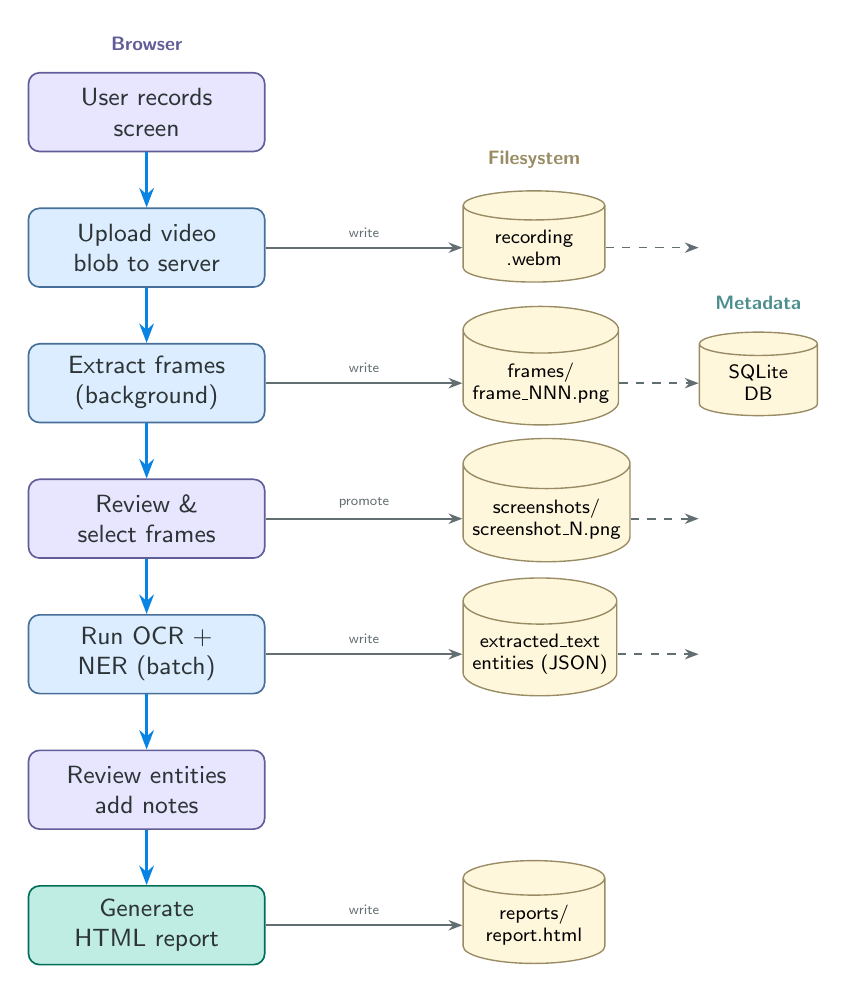
\begin{tikzpicture}[node distance=0.7cm]

    % Left column: User actions
    \node[sysblock=uifill, minimum width=3cm] (record) {User records\\screen};
    \node[sysblock=serverfill, minimum width=3cm, below=of record] (upload) {Upload video\\blob to server};
    \node[sysblock=serverfill, minimum width=3cm, below=of upload] (extract) {Extract frames\\(background)};
    \node[sysblock=uifill, minimum width=3cm, below=of extract] (review1) {Review \&\\select frames};
    \node[sysblock=serverfill, minimum width=3cm, below=of review1] (ocr) {Run OCR +\\NER (batch)};
    \node[sysblock=uifill, minimum width=3cm, below=of ocr] (review2) {Review entities\\add notes};
    \node[sysblock=acceptgreen, minimum width=3cm, below=of review2] (genreport) {Generate\\HTML report};

    % Right column: Data artifacts
    \node[storagenode, right=2.5cm of upload] (video) {recording\\{.webm}};
    \node[storagenode, right=2.5cm of extract] (frames) {frames/\\{frame\_NNN.png}};
    \node[storagenode, right=2.5cm of review1] (screenshots) {screenshots/\\{screenshot\_N.png}};
    \node[storagenode, right=2.5cm of ocr] (ocrdata) {extracted\_text\\entities (JSON)};
    \node[storagenode, right=2.5cm of genreport] (reportfile) {reports/\\{report.html}};

    % Center: DB
    \node[storagenode, minimum width=1.5cm, right=5.5cm of extract] (db) {SQLite\\DB};

    % Vertical flow
    \draw[bigarrow] (record) -- (upload);
    \draw[bigarrow] (upload) -- (extract);
    \draw[bigarrow] (extract) -- (review1);
    \draw[bigarrow] (review1) -- (ocr);
    \draw[bigarrow] (ocr) -- (review2);
    \draw[bigarrow] (review2) -- (genreport);

    % Horizontal: data written
    \draw[dataarrow] (upload.east) -- node[above, font=\tiny\sffamily] {write} (video.west);
    \draw[dataarrow] (extract.east) -- node[above, font=\tiny\sffamily] {write} (frames.west);
    \draw[dataarrow] (review1.east) -- node[above, font=\tiny\sffamily] {promote} (screenshots.west);
    \draw[dataarrow] (ocr.east) -- node[above, font=\tiny\sffamily] {write} (ocrdata.west);
    \draw[dataarrow] (genreport.east) -- node[above, font=\tiny\sffamily] {write} (reportfile.west);

    % DB connections
    \draw[dasharrow] (video.east) -- (db.west |- video.east);
    \draw[dasharrow] (frames.east) -- (db.west |- frames.east);
    \draw[dasharrow] (screenshots.east) -- (db.west |- screenshots.east);
    \draw[dasharrow] (ocrdata.east) -- (db.west |- ocrdata.east);

    % Labels
    \node[font=\scriptsize\sffamily\bfseries, text=uifill!60!black, above=0.15cm of record] {Browser};
    \node[font=\scriptsize\sffamily\bfseries, text=storagefill!60!black, above=0.15cm of video] {Filesystem};
    \node[font=\scriptsize\sffamily\bfseries, text=dbfill!60!black, above=0.15cm of db] {Metadata};

\end{tikzpicture}
\caption{Data flow from screen recording to final report, showing artifact creation at each stage.}
\end{figure}

\subsection{Entity-Relationship Diagram}

\begin{figure}[H]
\centering
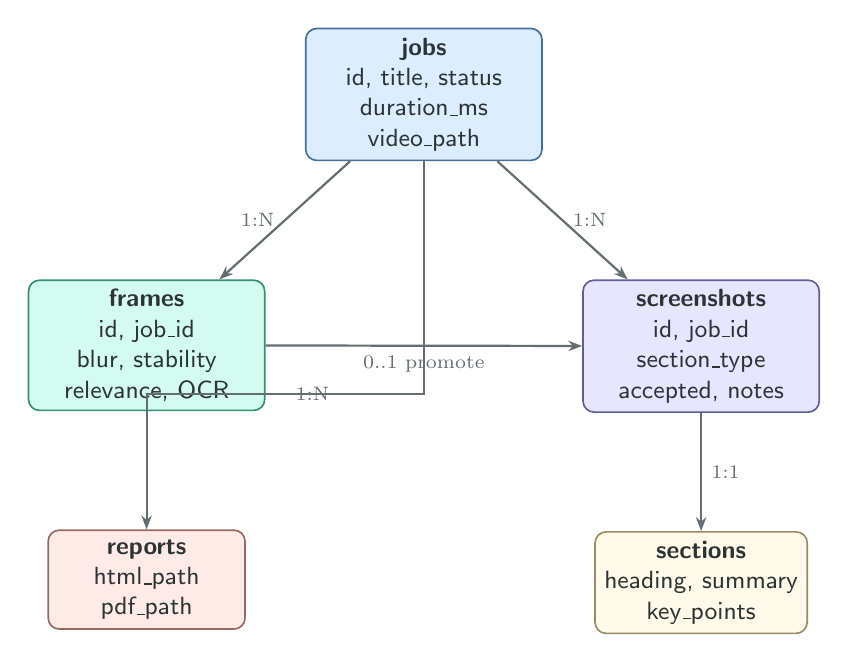
\begin{tikzpicture}[node distance=1.2cm and 2.5cm]

    % Entities
    \node[sysblock=serverfill, minimum width=3cm, minimum height=1.5cm] (jobs) {\textbf{jobs}\\id, title, status\\duration\_ms\\video\_path};
    \node[sysblock=pipelinefill, minimum width=3cm, minimum height=1.5cm, below left=1.5cm and 0.5cm of jobs] (frames) {\textbf{frames}\\id, job\_id\\blur, stability\\relevance, OCR};
    \node[sysblock=uifill, minimum width=3cm, minimum height=1.5cm, below right=1.5cm and 0.5cm of jobs] (screenshots) {\textbf{screenshots}\\id, job\_id\\section\_type\\accepted, notes};
    \node[sysblock=storagefill, minimum width=2.5cm, minimum height=1.2cm, below=1.5cm of screenshots] (sections) {\textbf{sections}\\heading, summary\\key\_points};
    \node[sysblock=threadfill, minimum width=2.5cm, minimum height=1.2cm, below=1.5cm of frames] (reports) {\textbf{reports}\\html\_path\\pdf\_path};

    % Relationships
    \draw[dataarrow] (jobs) -- node[left, font=\scriptsize] {1:N} (frames);
    \draw[dataarrow] (jobs) -- node[right, font=\scriptsize] {1:N} (screenshots);
    \draw[dataarrow] (frames) -- node[below, font=\scriptsize, sloped] {0..1 promote} (screenshots);
    \draw[dataarrow] (screenshots) -- node[right, font=\scriptsize] {1:1} (sections);
    \draw[dataarrow] (jobs) -- ++(0,-3.8) -| node[near start, right, font=\scriptsize] {1:N} (reports);

\end{tikzpicture}
\caption{Entity-relationship model. Frames are promoted to screenshots; each screenshot maps to one synthesized section.}
\end{figure}

\subsection{Data Flow Summary}

The system processes data through the following stages:

\begin{enumerate}
    \item \textbf{Capture:} User records screen via browser MediaRecorder API (WebM/MP4)
    \item \textbf{Upload:} Video blob uploaded to \codeinline{/api/jobs/\{id\}/upload}
    \item \textbf{Storage:} Saved in \codeinline{data/jobs/\{id\}/input/recording.webm}
    \item \textbf{Extraction:} User triggers \codeinline{POST /api/jobs/\{id\}/extract-frames}
    \item \textbf{Pipeline:} Background thread runs validation $\rightarrow$ sampling $\rightarrow$ scoring $\rightarrow$ scene detection $\rightarrow$ best-frame selection $\rightarrow$ deduplication
    \item \textbf{Frame Review:} User accepts/rejects frames, manually extracts additional ones
    \item \textbf{OCR:} User triggers \codeinline{POST /api/jobs/\{id\}/run-ocr} for text extraction
    \item \textbf{Entity Extraction:} Regex NER identifies dates, SSNs, currencies, etc.
    \item \textbf{Review:} User reviews OCR results, adds notes
    \item \textbf{Report:} Self-contained HTML evidence report generated
\end{enumerate}

% ════════════════════════════════════════════════════════════════════════════
\section{Project Structure}
% ════════════════════════════════════════════════════════════════════════════

\begin{lstlisting}[style=plain]
policycapture-local/
|
+-- apps/
|   +-- local_api/
|   |   +-- main.py              # FastAPI init, CORS, route mounting
|   |   +-- routes.py            # ALL API endpoints (~1200 lines)
|   |
|   +-- review-ui/
|       +-- templates/
|       |   +-- base.html        # Shared layout (nav, head, scripts)
|       |   +-- index.html       # Dashboard SPA shell
|       |   +-- recorder.html    # Screen recording page
|       |   +-- frame_review.html# Frame selection/review page
|       |   +-- ocr_review.html  # OCR results review page
|       |   +-- docs.html        # System documentation page
|       |
|       +-- static/
|           +-- css/styles.css   # All styles (~500 lines)
|           +-- js/
|           |   +-- app.js       # Dashboard SPA + API client (~1000 lines)
|           |   +-- recorder.js  # Screen capture logic (~400 lines)
|           |   +-- frame_review.js  # Frame review UI (~700 lines)
|           |   +-- ocr_review.js    # OCR review UI (~600 lines)
|           +-- img/logo.png     # Application logo
|
+-- packages/
|   +-- shared/
|   |   +-- config.py            # Configuration constants + env overrides
|   |   +-- database.py          # SQLite schema, CRUD (~340 lines)
|   |   +-- schemas.py           # Pydantic request/response models
|   |   +-- utils.py             # ID generation, path validation
|   |
|   +-- core/pipeline/
|       +-- orchestrator.py      # Full pipeline orchestration
|       +-- validate_video.py    # Format, size, readability checks
|       +-- sample_frames.py     # Timestamp-based frame extraction
|       +-- preprocess_frame.py  # Blur & stability scoring
|       +-- detect_relevance.py  # Keyword + visual structure detection
|       +-- scene_change.py      # Two-pass scene change detection
|       +-- choose_best_frame.py # Windowed best-frame selection
|       +-- dedupe_candidates.py # Perceptual hash deduplication
|       +-- classify_screenshot.py   # Rule-based section classification
|       +-- detect_elements.py   # Tesseract OCR + table detection
|       +-- extract_entities.py  # Regex NER (20+ entity types)
|       +-- synthesize_section.py# Summary & key-point generation
|       +-- generate_report.py   # HTML report generation
|       +-- medicaid_ner.py      # Experimental Medicaid-specific NER
|
+-- data/
|   +-- policycapture.db         # SQLite database
|   +-- jobs/{job_id}/           # Per-job artifact storage
|       +-- crop.json / input/ / frames/ / processed_frames/
|       +-- screenshots/ / reports/
|
+-- scripts/
|   +-- run.sh                   # Server startup script
|   +-- seed_demo.py             # Demo data seeding
|
+-- tests/test_pipeline.py       # Pipeline integration tests
+-- pyproject.toml               # Python project metadata + dependencies
+-- requirements.txt             # Pinned dependency list
+-- README.md                    # Quick-start guide
\end{lstlisting}

% ════════════════════════════════════════════════════════════════════════════
\section{Deployment Guide}
% ════════════════════════════════════════════════════════════════════════════

\subsection{Prerequisites}

\begin{tabularx}{\textwidth}{@{} l l X @{}}
    \toprule
    \textbf{Requirement} & \textbf{Version} & \textbf{Verification} \\
    \midrule
    Python & 3.11+ & \codeinline{python --version} \\
    pip & Latest & \codeinline{pip --version} \\
    Tesseract OCR & 4.x+ & \codeinline{tesseract --version} \\
    Disk Space & 2GB+ free & For video/frame storage \\
    \bottomrule
\end{tabularx}

\subsection{Step-by-Step Installation}

\subsubsection{1. Install System Dependencies}

\textbf{macOS (Homebrew):}
\begin{lstlisting}[style=bash]
brew install python@3.11 tesseract
\end{lstlisting}

\textbf{Ubuntu/Debian:}
\begin{lstlisting}[style=bash]
sudo apt update
sudo apt install python3.11 python3.11-venv tesseract-ocr
\end{lstlisting}

\textbf{Windows (WSL recommended):}
\begin{lstlisting}[style=bash]
# Inside WSL Ubuntu
sudo apt install python3.11 python3.11-venv tesseract-ocr
\end{lstlisting}

\subsubsection{2. Clone and Set Up the Project}

\begin{lstlisting}[style=bash]
git clone <repository-url>
cd policycapture-local

# Create virtual environment
python3.11 -m venv .venv
source .venv/bin/activate

# Install dependencies
pip install -r requirements.txt

# Or install from pyproject.toml with optional deps
pip install -e ".[dev,ocr]"
\end{lstlisting}

\subsubsection{3. Verify Installation}

\begin{lstlisting}[style=bash]
# Check Tesseract is accessible
tesseract --version

# Check Python packages
python -c "import cv2; print(cv2.__version__)"
python -c "import fastapi; print(fastapi.__version__)"
\end{lstlisting}

\subsubsection{4. Start the Server}

\begin{lstlisting}[style=bash]
bash scripts/run.sh
\end{lstlisting}

This executes:
\begin{lstlisting}[style=bash]
python -m uvicorn apps.local_api.main:app \
    --host 0.0.0.0 --port 8420 --reload
\end{lstlisting}

\begin{itemize}
    \item \codeinline{--host 0.0.0.0} --- Listens on all interfaces (for local access)
    \item \codeinline{--port 8420} --- Default port
    \item \codeinline{--reload} --- Auto-restarts on code changes (development mode)
\end{itemize}

\subsubsection{5. Open the Dashboard}

Navigate to \textbf{\url{http://localhost:8420}} in your browser.

\subsubsection{6. (Optional) Seed Demo Data}

\begin{lstlisting}[style=bash]
curl -X POST http://localhost:8420/api/demo/seed
\end{lstlisting}

Or click ``Seed Demo'' in the dashboard UI.

\subsection{Production Deployment Notes}

For a more hardened deployment (e.g., on a shared workstation):

\begin{lstlisting}[style=bash]
# Without --reload, with multiple workers
python -m uvicorn apps.local_api.main:app \
    --host 127.0.0.1 \
    --port 8420 \
    --workers 2

# Or with gunicorn (install separately)
pip install gunicorn
gunicorn apps.local_api.main:app \
    -w 2 \
    -k uvicorn.workers.UvicornWorker \
    --bind 127.0.0.1:8420
\end{lstlisting}

Key changes for production:
\begin{itemize}
    \item Bind to \codeinline{127.0.0.1} instead of \codeinline{0.0.0.0} to prevent network exposure
    \item Remove \codeinline{--reload} (saves CPU)
    \item Use 2+ workers for concurrent requests
    \item Consider running behind a reverse proxy (nginx) if network access is needed
\end{itemize}

% ════════════════════════════════════════════════════════════════════════════
\section{Configuration Reference}
% ════════════════════════════════════════════════════════════════════════════

All configuration lives in \filepath{packages/shared/config.py}. Every value can be overridden via environment variables.

\begin{longtable}{@{} p{3.8cm} p{3.2cm} l p{4.5cm} @{}}
    \toprule
    \textbf{Variable} & \textbf{Env Override} & \textbf{Default} & \textbf{Description} \\
    \midrule
    \endhead
    \codeinline{SERVER\_HOST} & \codeinline{PC\_HOST} & \codeinline{0.0.0.0} & Server bind address \\
    \codeinline{SERVER\_PORT} & \codeinline{PC\_PORT} & \codeinline{8420} & Server port \\
    \codeinline{FRAME\_SAMPLE\_INTERVAL\_SEC} & \codeinline{PC\_FRAME\_INTERVAL} & \codeinline{0.5} & Seconds between sampled frames \\
    \codeinline{RELEVANCE\_THRESHOLD} & \codeinline{PC\_RELEVANCE\_THRESHOLD} & \codeinline{0.3} & Min relevance score \\
    \codeinline{SIMILARITY\_THRESHOLD} & \codeinline{PC\_SIMILARITY\_THRESHOLD} & \codeinline{0.92} & Dedup threshold (higher = more aggressive) \\
    \codeinline{MAX\_FILE\_SIZE\_MB} & \codeinline{PC\_MAX\_FILE\_MB} & \codeinline{2048} & Max upload file size (MB) \\
    \codeinline{BLUR\_THRESHOLD} & --- & \codeinline{0.3} & Frames below this are rejected \\
    \codeinline{MIN\_CANDIDATE\_SCORE} & --- & \codeinline{0.2} & Min composite score \\
    \codeinline{BEST\_FRAME\_WINDOW\_SEC} & --- & \codeinline{4.0} & Time window for best-frame selection (s) \\
    \bottomrule
\end{longtable}

\subsection{Supported Video Formats}

\codeinline{.mp4}, \codeinline{.mov}, \codeinline{.avi}, \codeinline{.mkv}, \codeinline{.webm}

\subsection{Relevance Keywords}

The system looks for these keywords in extracted text to determine if a frame is relevant to policy/benefits review:

\begin{quote}
\texttt{demographics, income, household, members, eligibility, application, policy, address, amount, case number, benefits, enrollment, coverage, deductible, premium, copay, provider, plan, medicaid, medicare, snap, tanf, wic}
\end{quote}

\subsection{Section Types}

Frames are classified into these categories:

\begin{quote}
\texttt{demographics, income, household, eligibility, policy\_guidance, application\_step, table, unknown}
\end{quote}

% ════════════════════════════════════════════════════════════════════════════
\section{Database Design}
% ════════════════════════════════════════════════════════════════════════════

\subsection{Engine: SQLite with WAL Mode}

\textbf{Why SQLite?}
\begin{itemize}
    \item Zero configuration --- no server process, no connection strings
    \item Single file (\codeinline{data/policycapture.db}) --- easy to backup, move, reset
    \item WAL (Write-Ahead Logging) mode --- concurrent reads don't block writes
    \item Foreign keys enabled --- referential integrity enforced
    \item Perfect for single-user, local-first applications
\end{itemize}

\textbf{Thread Safety:}
\begin{itemize}
    \item Each thread gets its own connection via \codeinline{threading.local()}
    \item Connections are reused within the same thread
    \item \codeinline{check\_same\_thread=False} allows FastAPI's thread pool to share connections safely
\end{itemize}

\subsection{Schema}

\begin{lstlisting}[style=sql]
-- Core entity: a processing job tied to one video
CREATE TABLE jobs (
    id              TEXT PRIMARY KEY,     -- UUID
    title           TEXT NOT NULL,
    source_video_path TEXT,               -- Path to video file
    status          TEXT NOT NULL DEFAULT 'pending',
                    -- pending -> processing -> completed | failed
    duration_ms     INTEGER,              -- Video duration
    frame_count     INTEGER,              -- Total extracted frames
    screenshot_count INTEGER,             -- Selected screenshots
    created_at      TEXT NOT NULL,         -- ISO 8601 UTC
    updated_at      TEXT NOT NULL
);

-- Every frame sampled from the video
CREATE TABLE frames (
    id              TEXT PRIMARY KEY,
    job_id          TEXT NOT NULL REFERENCES jobs(id),
    frame_index     INTEGER NOT NULL,     -- Sequential index
    timestamp_ms    INTEGER NOT NULL,     -- Position in video
    source_image_path TEXT NOT NULL,      -- Path to PNG file
    blur_score      REAL DEFAULT 0,       -- 0.0 (blurry) to 1.0 (sharp)
    stability_score REAL DEFAULT 0,       -- 0.0 (changing) to 1.0 (static)
    relevance_score REAL DEFAULT 0,       -- 0.0 (irrelevant) to 1.0 (relevant)
    matched_keywords TEXT DEFAULT '[]',   -- JSON array
    extracted_text  TEXT DEFAULT '',      -- OCR text
    ocr_confidence  REAL DEFAULT 0,      -- 0.0 to 1.0
    candidate_score REAL DEFAULT 0       -- Composite score
);

-- Frames selected for the final report
CREATE TABLE screenshots (
    id              TEXT PRIMARY KEY,
    job_id          TEXT NOT NULL REFERENCES jobs(id),
    source_frame_id TEXT,                 -- FK to frames.id (nullable)
    image_path      TEXT NOT NULL,
    thumbnail_path  TEXT DEFAULT '',
    captured_at_ms  INTEGER DEFAULT 0,
    section_type    TEXT DEFAULT 'unknown',
    confidence      REAL DEFAULT 0,
    rationale       TEXT DEFAULT '',      -- Why this frame was selected
    matched_keywords TEXT DEFAULT '[]',
    extracted_text  TEXT DEFAULT '',
    accepted        INTEGER DEFAULT 1,    -- 0 = rejected, 1 = accepted
    notes           TEXT DEFAULT '',      -- User annotations
    order_index     INTEGER DEFAULT 0    -- Position in report
);

-- Synthesized report sections (one per screenshot)
CREATE TABLE sections (
    id              TEXT PRIMARY KEY,
    job_id          TEXT NOT NULL REFERENCES jobs(id),
    screenshot_id   TEXT REFERENCES screenshots(id),
    heading         TEXT DEFAULT '',
    section_type    TEXT DEFAULT 'unknown',
    summary         TEXT DEFAULT '',
    key_points      TEXT DEFAULT '[]',   -- JSON array
    confidence      REAL DEFAULT 0,
    final_order     INTEGER DEFAULT 0
);

-- Generated reports
CREATE TABLE reports (
    id              TEXT PRIMARY KEY,
    job_id          TEXT NOT NULL REFERENCES jobs(id),
    html_path       TEXT DEFAULT '',
    pdf_path        TEXT DEFAULT '',
    created_at      TEXT NOT NULL
);

-- Performance indexes
CREATE INDEX idx_frames_job ON frames(job_id);
CREATE INDEX idx_screenshots_job ON screenshots(job_id);
CREATE INDEX idx_sections_job ON sections(job_id);
\end{lstlisting}

\subsection{Entity Relationships}

\begin{lstlisting}[style=plain]
jobs (1) ---> (N) frames
jobs (1) ---> (N) screenshots
jobs (1) ---> (N) sections
jobs (1) ---> (N) reports
screenshots (1) ---> (1) sections
frames (1) ---> (0..1) screenshots  (via source_frame_id)
\end{lstlisting}

\subsection{How Data Flows Through Tables}

\begin{enumerate}
    \item \textbf{Job created} $\rightarrow$ \codeinline{jobs} row with status \codeinline{pending}
    \item \textbf{Video registered} $\rightarrow$ \codeinline{jobs.source\_video\_path} updated
    \item \textbf{Frames extracted} $\rightarrow$ \codeinline{frames} rows created (hundreds per video)
    \item \textbf{Frames scored} $\rightarrow$ \codeinline{frames.blur\_score}, \codeinline{relevance\_score}, etc. updated
    \item \textbf{Best frames selected} $\rightarrow$ \codeinline{screenshots} rows created from top \codeinline{frames}
    \item \textbf{User reviews} $\rightarrow$ \codeinline{screenshots.accepted}, \codeinline{screenshots.notes} updated
    \item \textbf{OCR runs} $\rightarrow$ \codeinline{screenshots.extracted\_text} populated
    \item \textbf{Sections synthesized} $\rightarrow$ \codeinline{sections} rows created
    \item \textbf{Report generated} $\rightarrow$ \codeinline{reports} row with path to HTML file
\end{enumerate}

% ════════════════════════════════════════════════════════════════════════════
\section{API Reference}
% ════════════════════════════════════════════════════════════════════════════

Base URL: \codeinline{http://localhost:8420}

\subsection{Job Management}

\begin{tabularx}{\textwidth}{@{} l l X @{}}
    \toprule
    \textbf{Method} & \textbf{Endpoint} & \textbf{Description} \\
    \midrule
    POST & \codeinline{/api/jobs} & Create a new job \\
    GET & \codeinline{/api/jobs} & List all jobs (newest first) \\
    GET & \codeinline{/api/jobs/\{id\}} & Get job details \\
    DELETE & \codeinline{/api/jobs/\{id\}} & Delete job + all data \\
    PATCH & \codeinline{/api/jobs/\{id\}/title} & Update job title \\
    POST & \codeinline{/api/jobs/\{id\}/auto-title} & Auto-generate title from OCR \\
    \bottomrule
\end{tabularx}

\vspace{0.5cm}

\textbf{Example --- Create Job:}
\begin{lstlisting}[style=json]
// Request: POST /api/jobs
{ "title": "March Eligibility Review" }

// Response:
{
  "id": "a1b2c3d4",
  "title": "March Eligibility Review",
  "status": "pending",
  "created_at": "2026-03-23T12:00:00Z"
}
\end{lstlisting}

\subsection{Video Registration}

\begin{tabularx}{\textwidth}{@{} l l X @{}}
    \toprule
    \textbf{Method} & \textbf{Endpoint} & \textbf{Description} \\
    \midrule
    POST & \codeinline{/api/jobs/\{id\}/upload} & Upload video (multipart form data) \\
    POST & \codeinline{/api/jobs/\{id\}/register-video} & Register local video path \\
    POST & \codeinline{/api/jobs/\{id\}/crop} & Store crop region \\
    GET & \codeinline{/api/jobs/\{id\}/video-info} & Get video metadata \\
    \bottomrule
\end{tabularx}

\vspace{0.5cm}

\textbf{Example --- Set Crop Region:}
\begin{lstlisting}[style=json]
// Request: POST /api/jobs/{id}/crop
{ "x": 100, "y": 50, "w": 1280, "h": 720 }
\end{lstlisting}

\subsection{Processing}

\begin{tabularx}{\textwidth}{@{} l l X @{}}
    \toprule
    \textbf{Method} & \textbf{Endpoint} & \textbf{Description} \\
    \midrule
    POST & \codeinline{/api/jobs/\{id\}/extract-frames} & Run frame extraction (background) \\
    POST & \codeinline{/api/jobs/\{id\}/process} & Run full pipeline (background) \\
    GET & \codeinline{/api/jobs/\{id\}/status} & Poll processing status \\
    \bottomrule
\end{tabularx}

\subsection{Frames \& Screenshots}

\begin{tabularx}{\textwidth}{@{} l l X @{}}
    \toprule
    \textbf{Method} & \textbf{Endpoint} & \textbf{Description} \\
    \midrule
    GET & \codeinline{/api/jobs/\{id\}/frames} & Get extracted frames \\
    GET & \codeinline{/api/jobs/\{id\}/screenshots} & Get selected screenshots \\
    PATCH & \codeinline{/api/screenshots/\{id\}} & Update screenshot metadata \\
    POST & \codeinline{/api/frames/\{id\}/promote} & Promote frame to screenshot \\
    POST & \codeinline{/api/jobs/\{id\}/extract-frame-at} & Extract frame at timestamp \\
    \bottomrule
\end{tabularx}

\subsection{OCR \& Entities}

\begin{tabularx}{\textwidth}{@{} l l X @{}}
    \toprule
    \textbf{Method} & \textbf{Endpoint} & \textbf{Description} \\
    \midrule
    POST & \codeinline{/api/jobs/\{id\}/run-ocr} & Run OCR + NER (batch, 4 workers) \\
    GET & \codeinline{/api/jobs/\{id\}/ocr-data} & Get all OCR results \\
    GET & \codeinline{/api/jobs/\{id\}/search?q=\{q\}} & Full-text search \\
    \bottomrule
\end{tabularx}

\subsection{Reports}

\begin{tabularx}{\textwidth}{@{} l l X @{}}
    \toprule
    \textbf{Method} & \textbf{Endpoint} & \textbf{Description} \\
    \midrule
    POST & \codeinline{/api/jobs/\{id\}/report} & Generate HTML report \\
    GET & \codeinline{/api/jobs/\{id\}/report} & Get report metadata \\
    GET & \codeinline{/api/jobs/\{id\}/report/html} & Get HTML content \\
    GET & \codeinline{/api/jobs/\{id\}/sections} & Get synthesized sections \\
    \bottomrule
\end{tabularx}

\subsection{File Serving \& Utilities}

\begin{tabularx}{\textwidth}{@{} l l X @{}}
    \toprule
    \textbf{Method} & \textbf{Endpoint} & \textbf{Description} \\
    \midrule
    GET & \codeinline{/api/artifacts/\{id\}/\{type\}/\{file\}} & Serve artifact files (sanitized) \\
    POST & \codeinline{/api/demo/seed} & Seed demo data \\
    \bottomrule
\end{tabularx}

% ════════════════════════════════════════════════════════════════════════════
\section{Processing Pipeline --- Deep Dive}
% ════════════════════════════════════════════════════════════════════════════

The pipeline is the heart of the system. Each stage is a Python module in \filepath{packages/core/pipeline/}.

\subsection{Stage 1: Video Validation}
\textit{Module: \filepath{validate\_video.py}}

Checks that the video file is valid before processing begins.

\textbf{Checks performed:}
\begin{itemize}
    \item File exists on disk
    \item Extension is in the supported set (\codeinline{.mp4}, \codeinline{.mov}, \codeinline{.avi}, \codeinline{.mkv}, \codeinline{.webm})
    \item File size $\leq$ 2\,GB (configurable via \codeinline{PC\_MAX\_FILE\_MB})
    \item OpenCV can open and read at least one frame
    \item Extracts metadata: FPS, frame count, duration
\end{itemize}

\textbf{WebM workaround:} Browser MediaRecorder often reports incorrect FPS (1000fps) for WebM. The validator detects this and falls back to seek-to-end duration measurement using \codeinline{CAP\_PROP\_POS\_MSEC}.

\subsection{Stage 2: Frame Sampling}
\textit{Module: \filepath{sample\_frames.py}}

Extracts frames from the video at regular intervals.

\textbf{Algorithm:}
\begin{enumerate}
    \item Opens video with OpenCV (\codeinline{cv2.VideoCapture})
    \item Seeks to timestamps at \codeinline{FRAME\_SAMPLE\_INTERVAL\_SEC} intervals (default: 0.5s)
    \item Uses \codeinline{CAP\_PROP\_POS\_MSEC} for seeking (not frame counting --- critical for WebM)
    \item Applies crop region from \codeinline{crop.json} if it exists
    \item Saves each frame as PNG in \codeinline{data/jobs/\{id\}/frames/}
    \item Creates 320$\times$180 thumbnails in \codeinline{data/jobs/\{id\}/processed\_frames/}
\end{enumerate}

\textbf{Adaptive sampling:}
\begin{itemize}
    \item Static sections (pixel correlation $>$ 0.995) $\rightarrow$ skip frames
    \item High-change sections (similarity $<$ 0.97) $\rightarrow$ increase sampling density
    \item Reduces frame count by 30--60\% on idle-heavy recordings
\end{itemize}

\subsection{Stage 3: Preprocessing}
\textit{Module: \filepath{preprocess\_frame.py}}

Computes quality scores for each frame.

\textbf{Blur Score:}
\begin{equation}
    \text{blur\_score} = \min\!\left(\frac{\text{Var}(\text{Laplacian}(I))}{5000},\; 1.0\right)
\end{equation}

\begin{itemize}
    \item Laplacian operator detects edges; variance measures edge strength
    \item High variance = sharp image, low variance = blurry
    \item Threshold: $\geq 0.15$ is considered ``sharp enough''
\end{itemize}

\textbf{Stability Score:}
\begin{equation}
    \text{stability} = 1.0 - \frac{\text{MSE}(I_t, I_{t-1})}{255^2}
\end{equation}

\begin{itemize}
    \item MSE = mean squared error between current and previous frame (grayscale)
    \item A perfectly static screen scores 1.0
\end{itemize}

\subsection{Stage 4: Relevance Detection}
\textit{Module: \filepath{detect\_relevance.py}}

Determines how relevant each frame is to the policy/benefits review task by combining two signals:

\textbf{Keyword Score (70\% weight):}
\begin{equation}
    \text{keyword\_score} = \min\!\left(\frac{\text{matched\_count}}{23 \times 0.3},\; 1.0\right)
\end{equation}

\textbf{Structure Score (30\% weight):}
\begin{equation}
    \text{structure\_score} = 0.6 \times \text{horizontal\_lines} + 0.4 \times \text{vertical\_lines}
\end{equation}

\textbf{Combined Relevance:}
\begin{equation}
    \text{relevance} = 0.7 \times \text{keyword\_score} + 0.3 \times \text{structure\_score}
\end{equation}

Frames below \codeinline{RELEVANCE\_THRESHOLD} (0.3) are dropped.

\subsection{Stage 5: Scene Change Detection}
\label{sec:adaptive}
\textit{Module: \filepath{scene\_change.py}}

Identifies frames where the visual content changes significantly (new page, new screen, scroll). Uses a \textbf{two-pass approach} for speed.

\textbf{Pass 1 --- Perceptual Hash (fast pre-filter):}
\begin{itemize}
    \item Compute DCT-based perceptual hash (16$\times$16 grid) for each frame
    \item Compare adjacent frames by Hamming distance
    \item Frames with high similarity quickly ruled out ($< 1$ms per comparison)
\end{itemize}

\textbf{Pass 2 --- SSIM + Histogram (accurate, selective):}
\begin{equation}
    \text{similarity} = 0.65 \times \text{SSIM} + 0.35 \times \text{histogram\_correlation}
\end{equation}

\begin{itemize}
    \item Only run on ``ambiguous'' frames from Pass 1
    \item Threshold: similarity $< 0.92$ = scene change
    \item Typically runs on only 20--40\% of frames
\end{itemize}

\textbf{Why two passes?} Pure SSIM costs 50--100ms per comparison. The perceptual hash pre-filter eliminates obvious non-changes in $< 1$ms, giving a net 2--3$\times$ speedup.

\subsection{Stage 6: Best Frame Selection}
\textit{Module: \filepath{choose\_best\_frame.py}}

From all frames that passed quality and relevance filters, selects the single best frame for each time window.

\textbf{Candidate Composite Score:}
\begin{equation}
    \text{candidate\_score} = 0.35 \times \text{blur} + 0.45 \times \text{relevance} + 0.20 \times \text{stability}
\end{equation}

\begin{enumerate}
    \item Group frames into 4-second windows (configurable via \codeinline{BEST\_FRAME\_WINDOW\_SEC})
    \item Select the frame with the highest composite score in each window
    \item These become the ``candidate screenshots''
\end{enumerate}

\subsection{Stage 7: Deduplication}
\textit{Module: \filepath{dedupe\_candidates.py}}

Removes near-duplicate frames across different time windows.

\begin{itemize}
    \item Compute perceptual hash for each candidate frame
    \item Compare all pairs; if similarity $\geq 0.92$, mark the lower-scored frame as duplicate
    \item Duplicate frames get \codeinline{candidate\_score = 0.0}
\end{itemize}

\subsection{Stage 8: OCR \& Element Detection}
\textit{Module: \filepath{detect\_elements.py}}

Extracts text and detects tables from screenshots using \textbf{multi-strategy OCR preprocessing}:

\begin{longtable}{@{} l l l @{}}
    \toprule
    \textbf{Strategy} & \textbf{Technique} & \textbf{Best For} \\
    \midrule
    Standard & Denoise $\rightarrow$ CLAHE $\rightarrow$ sharpen & Clean screen captures \\
    Otsu & Global binarization & High-contrast documents \\
    Adaptive & Local threshold (block size 11) & Uneven lighting, gradients \\
    Heavy & 3$\times$ upscale $\rightarrow$ aggressive denoise $\rightarrow$ deskew & Low-resolution captures \\
    \bottomrule
\end{longtable}

\textbf{Tesseract Configuration:}
\begin{itemize}
    \item Page Segmentation Mode 3 (fully automatic page segmentation)
    \item TSV output for structured data (block, paragraph, line, word positions)
    \item Words below 30\% confidence are discarded
\end{itemize}

\textbf{Table Detection:}
\begin{enumerate}
    \item Detect horizontal and vertical grid lines (morphological operations)
    \item Find line intersections to determine cell boundaries
    \item Run per-cell OCR within detected boundaries
    \item Output structured table data (rows $\times$ columns $\times$ text)
\end{enumerate}

\textbf{Parallelism:} Uses \codeinline{ThreadPoolExecutor} with 4 workers for batch processing.

\subsection{Stage 9: Entity Extraction}
\textit{Module: \filepath{extract\_entities.py}}

Identifies structured entities in OCR text using 20+ regex patterns.

\begin{longtable}{@{} l p{10cm} @{}}
    \toprule
    \textbf{Category} & \textbf{Entity Types} \\
    \midrule
    \endhead
    Dates/Times & \codeinline{date} (MM/DD/YYYY, YYYY-MM-DD, Month DD YYYY, etc.), \codeinline{time\_value} \\
    Identifiers & \codeinline{ssn}, \codeinline{ein}, \codeinline{npi}, \codeinline{policy\_number}, \codeinline{case\_number}, \codeinline{claim\_number}, \codeinline{group\_number}, \codeinline{account\_number}, \codeinline{id\_number} \\
    Financial & \codeinline{currency} (\$, USD, EUR, GBP), \codeinline{percentage} \\
    Contact & \codeinline{phone}, \codeinline{email}, \codeinline{url} \\
    Location & \codeinline{address}, \codeinline{zip\_code}, \codeinline{state} \\
    Identity & \codeinline{person\_name} (title-case heuristic), \codeinline{organization} \\
    Medical & \codeinline{medical\_code} (ICD, CPT, HCPCS patterns) \\
    \bottomrule
\end{longtable}

\textbf{Special Features:}
\begin{itemize}
    \item \textbf{Overlapping deduplication:} If multiple patterns match the same text span, the most specific one wins
    \item \textbf{PII masking:} SSNs displayed as \codeinline{***-**-XXXX}
    \item \textbf{Form field detection:} Extracts key-value pairs from form-style text
    \item \textbf{List extraction:} Detects bulleted, numbered, and lettered lists
    \item \textbf{Section header detection:} Identifies section headings by formatting patterns
\end{itemize}

\subsection{Stage 10: Classification}
\textit{Module: \filepath{classify\_screenshot.py}}

Assigns each screenshot to a section type using rule-based keyword matching.

\begin{tabularx}{\textwidth}{@{} l X @{}}
    \toprule
    \textbf{Section Type} & \textbf{Trigger Keywords} \\
    \midrule
    demographics & name, address, date of birth, ssn, contact, phone, email \\
    income & income, wages, salary, employment, employer, pay stub \\
    household & household, members, dependents, family size, spouse \\
    eligibility & eligible, eligibility, qualify, determination, approved, denied \\
    \bottomrule
\end{tabularx}

\subsection{Stage 11: Synthesis}
\textit{Module: \filepath{synthesize\_section.py}}

Generates a heading, summary, and key points for each screenshot section (heuristic-based, no LLM):
\begin{itemize}
    \item Heading derived from section type (``Demographics Information'', ``Income Verification'', etc.)
    \item Summary: first 200 characters of extracted text, cleaned
    \item Key points: matched keywords formatted as bullet points
    \item Ordering weight: 10--99 based on section type priority
\end{itemize}

\subsection{Stage 12: Report Generation}
\textit{Module: \filepath{generate\_report.py}}

Produces a self-contained HTML evidence report:
\begin{itemize}
    \item Images embedded as base64 data URIs (no external file references)
    \item Professional blue/gray theme, card-based layout
    \item Sections ordered by \codeinline{final\_order}
    \item PDF generation is stubbed out (extension point for ReportLab/weasyprint)
\end{itemize}

% ════════════════════════════════════════════════════════════════════════════
\section{Frontend Architecture}
% ════════════════════════════════════════════════════════════════════════════

\subsection{Routing Model}

The frontend uses a \textbf{hybrid routing} approach:

\begin{tabularx}{\textwidth}{@{} l l X @{}}
    \toprule
    \textbf{Route} & \textbf{Type} & \textbf{File} \\
    \midrule
    \codeinline{/} & Jinja2 template $\rightarrow$ SPA & \filepath{index.html} + \filepath{app.js} \\
    \codeinline{/\#/} & Hash route (job list) & \filepath{app.js} \\
    \codeinline{/\#/jobs/\{id\}} & Hash route (job detail) & \filepath{app.js} \\
    \codeinline{/\#/jobs/\{id\}/report} & Hash route (report view) & \filepath{app.js} \\
    \codeinline{/recorder} & Jinja2 template page & \filepath{recorder.html} + \filepath{recorder.js} \\
    \codeinline{/jobs/\{id\}/frames} & Jinja2 template page & \filepath{frame\_review.html} + \filepath{frame\_review.js} \\
    \codeinline{/jobs/\{id\}/ocr-review} & Jinja2 template page & \filepath{ocr\_review.html} + \filepath{ocr\_review.js} \\
    \codeinline{/docs} & Jinja2 template page & \filepath{docs.html} \\
    \bottomrule
\end{tabularx}

\subsection{app.js --- Dashboard SPA ($\sim$1000 lines)}

\begin{itemize}
    \item \codeinline{API} object: centralized fetch wrapper for all API calls
    \item Toast notification system for success/error feedback
    \item Hash router: parses \codeinline{window.location.hash} to render views
    \item Job list, job detail, and report views
    \item Modal system for create/rename job dialogs
\end{itemize}

\subsection{recorder.js --- Screen Capture ($\sim$400 lines)}

\begin{itemize}
    \item \codeinline{navigator.mediaDevices.getDisplayMedia()} for screen sharing
    \item Live preview with interactive crop overlay
    \item Coordinate transformation: screen CSS pixels $\rightarrow$ video pixel coordinates (DPI-aware)
    \item MediaRecorder codec negotiation: MP4 $>$ WebM VP9 $>$ WebM VP8
    \item Records to Blob, uploads via \codeinline{POST /api/jobs/\{id\}/upload}
\end{itemize}

\subsection{frame\_review.js --- Frame Selection ($\sim$700 lines)}

\begin{itemize}
    \item Timeline visualization: continuous horizontal scrubber
    \item Color-coded markers: \textcolor{green!60!black}{green} = auto-selected, \textcolor{blue}{blue} = manual, \textcolor{orange}{orange} = scene change, \textcolor{gray}{gray} = redundant
    \item Thumbnail gallery with confidence score badges
    \item Actions: promote, remove, extract at timestamp
    \item Keyboard shortcuts: arrow keys (navigate), Space (select/deselect), Escape (close)
\end{itemize}

\subsection{ocr\_review.js --- OCR Results ($\sim$600 lines)}

\begin{itemize}
    \item Frame strip: horizontal scrollable screenshot strip
    \item Tabbed content: Text, Entities, Tables, Notes
    \item Entity highlighting with color-coded badges by type
    \item Entity filter chips and full-text search
    \item Export to JSON
\end{itemize}

\subsection{styles.css --- Unified Styling ($\sim$500 lines)}

\begin{itemize}
    \item CSS custom properties for theming
    \item Primary color: \texttt{\#0984e3} (blue), Dark: \texttt{\#2d3436} (charcoal)
    \item Card-based layout with subtle shadows
    \item Badge system, modal overlays, timeline/gallery grids
    \item Responsive: mobile-first with breakpoints
\end{itemize}

% ════════════════════════════════════════════════════════════════════════════
\section{Algorithms \& Scoring}
% ════════════════════════════════════════════════════════════════════════════

\subsection{Blur Detection}

\begin{equation}
    \text{blur\_score} = \min\!\left(\frac{\text{Var}\bigl(\nabla^2 I\bigr)}{5000},\; 1.0\right)
\end{equation}

\begin{tabularx}{\textwidth}{@{} l X @{}}
    \toprule
    \textbf{Range} & \textbf{Interpretation} \\
    \midrule
    $0.00 - 0.15$ & Blurry (rejected) \\
    $0.15 - 0.40$ & Acceptable \\
    $0.40 - 1.00$ & Sharp \\
    \bottomrule
\end{tabularx}

\subsection{Frame Stability}

\begin{equation}
    \text{stability} = 1.0 - \frac{\frac{1}{N}\sum_{i}(I^{(t)}_i - I^{(t-1)}_i)^2}{255^2}
\end{equation}

\begin{tabularx}{\textwidth}{@{} l X @{}}
    \toprule
    \textbf{Score} & \textbf{Interpretation} \\
    \midrule
    $1.00$ & Identical frames (static screen) \\
    $0.95$ & Minor change (cursor move, animation) \\
    $0.70$ & Significant change (scroll, navigation) \\
    $< 0.50$ & Major scene change \\
    \bottomrule
\end{tabularx}

\subsection{Relevance Scoring}

\begin{equation}
    \text{relevance} = 0.7 \times \min\!\left(\frac{|\text{matches}|}{23 \times 0.3}, 1.0\right) + 0.3 \times \bigl(0.6h + 0.4v\bigr)
\end{equation}

where $h$ = horizontal line ratio, $v$ = vertical line ratio.

\subsection{Scene Change Detection}

\begin{align}
    \text{Pass 1:}\quad & \text{phash\_sim} = 1 - \frac{\text{hamming}(h_t, h_{t-1})}{|\text{bits}|} \\[6pt]
    \text{Pass 2:}\quad & \text{combined} = 0.65 \times \text{SSIM} + 0.35 \times \text{hist\_corr} \\[6pt]
    & \text{Scene change if } \text{combined} < 0.92
\end{align}

\subsection{Candidate Scoring}

\begin{equation}
    \text{candidate\_score} = 0.35 \cdot \text{blur} + 0.45 \cdot \text{relevance} + 0.20 \cdot \text{stability}
\end{equation}

\subsection{Redundancy Detection}

\begin{equation}
    \text{If } \text{SSIM}(I_i, I_j) > 0.95 \implies I_j \text{ is redundant (lower-scored frame dropped)}
\end{equation}

% ════════════════════════════════════════════════════════════════════════════
\section{Key Implementation Details}
% ════════════════════════════════════════════════════════════════════════════

\subsection{WebM Compatibility}

The browser's MediaRecorder API primarily produces WebM video with VP8 or VP9 codecs. OpenCV's WebM support has a known issue: \codeinline{CAP\_PROP\_FPS} often returns 1000.0 instead of the actual framerate. PolicyCapture handles this:

\begin{enumerate}
    \item \textbf{Detection:} If reported FPS $> 120$, it's likely wrong
    \item \textbf{Duration fallback:} Seek to end of video, read \codeinline{CAP\_PROP\_POS\_MSEC} for actual duration
    \item \textbf{Frame extraction:} Uses \codeinline{CAP\_PROP\_POS\_MSEC} for seeking (not frame counting) --- always works correctly regardless of FPS metadata
\end{enumerate}

\subsection{Crop Region Handling}

Crop is deliberately \textbf{not} applied during recording:
\begin{itemize}
    \item Full screen is always captured (for smooth playback and potential re-cropping)
    \item Crop region stored as \codeinline{\{x, y, w, h\}} in video pixel coordinates
    \item Applied server-side during \codeinline{sample\_frames} using NumPy array slicing
    \item Coordinate transformation in \filepath{recorder.js} handles DPI scaling between CSS pixels and video pixels
\end{itemize}

\subsection{Background Processing}

Long-running operations (frame extraction, OCR) run in Python background threads (\codeinline{threading.Thread}). The API returns immediately and clients poll \codeinline{GET /api/jobs/\{id\}/status}. This avoids HTTP timeout issues and allows the user to continue interacting with the UI.

\subsection{File Organization}

Each job gets an isolated directory:

\begin{lstlisting}[style=plain]
data/jobs/{uuid}/
  crop.json               # Crop region (optional)
  input/                  # Source video
    recording.webm
  frames/                 # ALL sampled frames
    frame_000.png
    frame_001.png
    ...
  processed_frames/       # Thumbnails (320x180)
    frame_000.png
    ...
  screenshots/            # Selected frames
    screenshot_001.png
    ...
  reports/                # Generated reports
    report.html
\end{lstlisting}

\subsection{ID Generation}

All IDs are UUIDs generated by \filepath{packages/shared/utils.py}. This ensures uniqueness across jobs, frames, screenshots, and sections without coordination.

\subsection{Path Sanitization}

The artifact serving endpoint (\codeinline{/api/artifacts/\{id\}/\{type\}/\{file\}}) sanitizes file paths to prevent directory traversal attacks. Only allowed subdirectories (\codeinline{frames}, \codeinline{processed\_frames}, \codeinline{screenshots}, \codeinline{reports}, \codeinline{input}) can be accessed.

% ════════════════════════════════════════════════════════════════════════════
\section{User Workflow --- End to End}
% ════════════════════════════════════════════════════════════════════════════

\subsection{Step 1: Create a Job}

Open \url{http://localhost:8420}. Click \textbf{``New Job''}. Enter a title (e.g., ``March SNAP Eligibility Review''). This creates a \codeinline{jobs} row with status \codeinline{pending}.

\subsection{Step 2: Record the Screen}

Click \textbf{``Record''} on the job card. This opens the Recorder page.

\begin{enumerate}
    \item Click \textbf{``Start Recording''} $\rightarrow$ browser requests screen sharing permission
    \item Select the screen/window to capture
    \item (Optional) Drag on the preview to define a crop region
    \item Navigate through the policy/benefits system while recording
    \item Click \textbf{``Stop Recording''}
    \item The video blob is uploaded to the server automatically
\end{enumerate}

\subsection{Step 3: Extract Frames}

Click \textbf{``Extract Frames''}. The pipeline runs in the background:

\begin{enumerate}
    \item Validates the video
    \item Samples frames every 0.5 seconds
    \item Scores each frame for blur, stability, and relevance
    \item Detects scene changes
    \item Selects the best frame per 4-second window
    \item Removes near-duplicates
\end{enumerate}

You're redirected to the \textbf{Frame Review} page.

\subsection{Step 4: Review Frames}

The Frame Review page shows a timeline scrubber with color-coded markers, a thumbnail gallery, and a side panel with auto-selected/manual frames.

\textbf{Actions available:}
\begin{itemize}
    \item Click a frame to view full-size
    \item Click checkmark to accept/reject
    \item Use timeline to navigate to a specific moment
    \item Click ``Extract Frame'' for manual extraction at any timestamp
    \item Arrow keys to navigate, Space to select/deselect
\end{itemize}

\subsection{Step 5: Run OCR}

On the OCR Review page, click \textbf{``Run OCR \& Extract''}. This processes all selected screenshots through multi-strategy OCR, entity extraction, table detection, and section classification.

\subsection{Step 6: Review Results}

Browse results across four tabs:
\begin{itemize}
    \item \textbf{Text tab:} Raw OCR output
    \item \textbf{Entities tab:} Extracted entities with color-coded badges
    \item \textbf{Tables tab:} Detected tables rendered as HTML
    \item \textbf{Notes tab:} Free-form annotations
\end{itemize}

\subsection{Step 7: Generate Report}

Click \textbf{``Generate Report''} to produce a self-contained HTML evidence report with embedded screenshots, section headings, summaries, and extracted key points.

\subsection{Step 8: Export}

\begin{itemize}
    \item Download the HTML report (self-contained, no external dependencies)
    \item Export OCR data as JSON for integration with other systems
\end{itemize}

% ════════════════════════════════════════════════════════════════════════════
\section{Extension Points}
% ════════════════════════════════════════════════════════════════════════════

The codebase is designed to be modular. These are the marked extension points:

\begin{longtable}{@{} p{3.5cm} p{3.5cm} p{3.5cm} p{3.5cm} @{}}
    \toprule
    \textbf{Extension} & \textbf{File} & \textbf{Current} & \textbf{Upgrade To} \\
    \midrule
    \endhead
    OCR Engine & \filepath{detect\_elements.py} & Tesseract (subprocess) & PaddleOCR, EasyOCR, Azure Doc Intelligence, AWS Textract \\[6pt]
    NER & \filepath{extract\_entities.py} & 20+ regex patterns & SpaCy, GLiNER, fine-tuned transformer \\[6pt]
    Classification & \filepath{classify\_screenshot.py} & Keyword rules & Fine-tuned image classifier or multimodal model \\[6pt]
    Synthesis & \filepath{synthesize\_section.py} & Heuristic summarization & Claude API for intelligent summaries \\[6pt]
    PDF Generation & \filepath{generate\_report.py} & HTML only (PDF stubbed) & ReportLab or weasyprint \\[6pt]
    Screen Capture & New component & Browser MediaRecorder & Chrome extension feeding same pipeline \\
    \bottomrule
\end{longtable}

\textbf{Note:} \filepath{medicaid\_ner.py} contains an experimental Medicaid-specific NER module that can be integrated as an additional entity extraction layer.

% ════════════════════════════════════════════════════════════════════════════
\section{Troubleshooting}
% ════════════════════════════════════════════════════════════════════════════

\subsection{Server Won't Start}

\textbf{Error:} \codeinline{ERROR: [Errno 48] Address already in use}

Port 8420 is occupied. Kill the existing process:
\begin{lstlisting}[style=bash]
lsof -i :8420
kill -9 <PID>
\end{lstlisting}

Or change the port:
\begin{lstlisting}[style=bash]
PC_PORT=8421 bash scripts/run.sh
\end{lstlisting}

\subsection{Tesseract Not Found}

\textbf{Error:} \codeinline{FileNotFoundError: tesseract is not installed or not in PATH}

\begin{lstlisting}[style=bash]
brew install tesseract          # macOS
sudo apt install tesseract-ocr  # Ubuntu
\end{lstlisting}

\subsection{OCR Returns Empty Text}

\begin{itemize}
    \item Check that the screenshot has readable text (not just graphics)
    \item Verify Tesseract language packs: \codeinline{tesseract --list-langs}
    \item Try increasing frame resolution (reduce crop area)
    \item Check blur score --- very blurry frames produce poor OCR
\end{itemize}

\subsection{Video Won't Process}

\begin{itemize}
    \item Ensure the file is one of: \codeinline{.mp4}, \codeinline{.mov}, \codeinline{.avi}, \codeinline{.mkv}, \codeinline{.webm}
    \item File size must be $< 2$\,GB
    \item Verify OpenCV can read it: \codeinline{python -c "import cv2; print(cv2.VideoCapture('path').isOpened())"}
\end{itemize}

\subsection{Frames Are All Blurry}

\begin{itemize}
    \item Reduce \codeinline{PC\_FRAME\_INTERVAL} to sample more frequently (e.g., \codeinline{0.25})
    \item Lower \codeinline{BLUR\_THRESHOLD} in \filepath{config.py} to accept slightly blurry frames
    \item Ensure the source recording was at reasonable resolution
\end{itemize}

\subsection{Database Is Locked}

SQLite WAL mode handles most concurrency, but if you see ``database is locked'':
\begin{itemize}
    \item Kill any zombie server processes
    \item Delete \codeinline{data/policycapture.db-wal} and \codeinline{data/policycapture.db-shm} (they regenerate)
    \item Restart the server
\end{itemize}

\subsection{WebM FPS Issues}

If frame extraction produces wrong timestamps, this is the WebM FPS bug. The code handles it automatically, but if issues persist:
\begin{itemize}
    \item Try recording in MP4 instead (Safari supports this)
    \item Or re-encode: \codeinline{ffmpeg -i input.webm -c:v libx264 output.mp4}
\end{itemize}

% ════════════════════════════════════════════════════════════════════════════
\section{Performance Characteristics}
% ════════════════════════════════════════════════════════════════════════════

\subsection{Processing Times}

\begin{tabularx}{\textwidth}{@{} l l X @{}}
    \toprule
    \textbf{Operation} & \textbf{Typical Time} & \textbf{Notes} \\
    \midrule
    Frame sampling (1 min video) & 3--8 seconds & Depends on resolution and interval \\
    Blur/stability scoring & $< 1$ms per frame & Pure NumPy \\
    Relevance detection & 10--50ms per frame & Includes lightweight OCR \\
    Scene change (Pass 1 --- phash) & $< 1$ms per comparison & DCT-based hash \\
    Scene change (Pass 2 --- SSIM) & 50--100ms per comparison & Only on ambiguous frames \\
    Tesseract OCR & 50--200ms per frame & Depends on content density \\
    Entity extraction & $< 10$ms per frame & Pure regex \\
    Table detection & 100--500ms per frame & Only on frames with grid lines \\
    Report generation & $< 1$ second & HTML with base64 images \\
    \midrule
    \textbf{Full pipeline (1 min video)} & \textbf{15--45 seconds} & \textbf{End to end} \\
    \textbf{Full pipeline (5 min video)} & \textbf{60--180 seconds} & \textbf{Depends on content variety} \\
    \bottomrule
\end{tabularx}

\subsection{Storage Requirements}

\begin{tabularx}{\textwidth}{@{} l l X @{}}
    \toprule
    \textbf{Asset} & \textbf{Size per Frame} & \textbf{Notes} \\
    \midrule
    Full frame PNG & 200--800 KB & 1920$\times$1080 typical \\
    Thumbnail PNG & 15--30 KB & 320$\times$180 \\
    Total per minute of video & 50--200 MB & At 0.5s sampling interval \\
    \bottomrule
\end{tabularx}

% ════════════════════════════════════════════════════════════════════════════
\section{Security Considerations}
% ════════════════════════════════════════════════════════════════════════════

\subsection{PII Handling}

\begin{itemize}
    \item \textbf{All data stays local.} No network calls, no telemetry, no cloud storage.
    \item SSNs are masked in the entity extraction output (\codeinline{***-**-XXXX})
    \item The database and artifact files should be protected by OS-level file permissions
\end{itemize}

\subsection{Path Traversal Protection}

The artifact serving endpoint sanitizes file paths:
\begin{itemize}
    \item Only allows access to known subdirectories (\codeinline{frames}, \codeinline{screenshots}, etc.)
    \item Rejects paths containing \codeinline{..} or absolute paths
    \item Job IDs are validated as UUIDs
\end{itemize}

\subsection{Input Validation}

\begin{itemize}
    \item Video file sizes are capped (default 2\,GB)
    \item Video formats are allowlisted
    \item Pydantic models validate all API request bodies
    \item File uploads use multipart form data (not raw body)
\end{itemize}

\subsection{No Authentication}

This is intentional. The server is designed to run on \codeinline{localhost} for a single user. If you need multi-user access:
\begin{itemize}
    \item Add an authentication middleware to FastAPI
    \item Bind to \codeinline{127.0.0.1} instead of \codeinline{0.0.0.0}
    \item Put a reverse proxy (nginx + basic auth) in front
\end{itemize}

\subsection{CORS}

CORS is configured to allow all origins (\codeinline{*}) for local development. Tighten this if deploying on a network.

% ════════════════════════════════════════════════════════════════════════════
\vfill
\begin{center}
\textcolor{primary}{\rule{0.6\textwidth}{1.5pt}}\\[12pt]
{\small\textcolor{commentgray}{This guide covers the complete PolicyCapture Local system as of March 2026.\\
For questions or contributions, see the project repository.}}
\end{center}

\end{document}
